\documentclass[slidescentered]{beamer}
\usepackage[english]{babel}
\usepackage[utf8x]{inputenc}
\usepackage[T1]{fontenc}
\usepackage{lmodern}
\usepackage{fix-cm}
\usepackage{color}
\usepackage{graphicx}
\usepackage{hyperref}
\usepackage{listings}

\hypersetup{
    colorlinks=true,
    linkcolor=blue,
    filecolor=magenta,      
    urlcolor=cyan,
    pdftitle={Overleaf Example},
    pdfpagemode=FullScreen,
    }

\usetheme{UniboTesi}

\title{Artificial Intelligence in Industry Project}
\subtitle{Forecasting Median House Prices}
\date{\today}
\department{Computer Science and Engineering}
\degree{Master Degree in Artificial Intelligence}

\begin{document}

%------------------------------------------------
\begin{frame}[noframenumbering]
    \titlepage
\end{frame}

%------------------------------------------------
\begin{frame}{Project Objective}

    \begin{itemize}

        \item Predict monthly median house prices using historical property sales data
        \item Data source: \href{https://www.kaggle.com/datasets/htagholdings/property-sales}{Kaggle property sales time series dataset}

        \item Understand which factors drive price dynamics over time

        \item Compare multiple forecasting approaches

        \item Investigate unexpected model behaviour and improve the feature space

    \end{itemize}

\end{frame}

%------------------------------------------------
\begin{frame}{Dataset}

    \begin{itemize}

        \item Data source: Kaggle property sales dataset

        \item Time span: 2007 -- 2019

        \item Each observation corresponds to a property sale

        \item Key variables:

              \begin{itemize}
                  \item sale date
                  \item property price
                  \item property type (house / unit)
                  \item number of bedrooms
                  \item postcode
              \end{itemize}

        \item Goal: predict a \textbf{monthly time series of housing prices}

    \end{itemize}

\end{frame}

%------------------------------------------------

\begin{frame}{Project outline}

    \begin{itemize}
        \item Problem \& dataset
        \item Extensive EDA
        \item Data issues and preprocessing (missing values and outliers)
        \item Feature engineering
        \item ML models evaluation
        \item Feature importance analysis
        \item Observations of results and hypothesis exploration
    \end{itemize}

\end{frame}
%------------------------------------------------


\begin{frame}{Dataset}
    \addtolength{\tabcolsep}{-4.5pt}
    \begin{tabular}{|c|c|c|c|c|c|}
        \hline
        \textbf{Index} & \textbf{datesold} & \textbf{postcode} & \textbf{price} & \textbf{propertyType} & \textbf{bedrooms} \\ \hline
        0              & 2007-02-07        & 2607              & 525000         & house                 & 4                 \\ \hline
        1              & 2007-02-27        & 2906              & 290000         & house                 & 3                 \\ \hline
        2              & 2007-03-07        & 2905              & 328000         & house                 & 3                 \\ \hline
        3              & 2007-03-09        & 2905              & 380000         & house                 & 4                 \\ \hline
        4              & 2007-03-21        & 2906              & 310000         & house                 & 3                 \\ \hline
    \end{tabular}
    \vspace{1.5em}
    \begin{itemize}

        \item Each row corresponds to a transaction

        \item Dataset contains thousands of observations

        \item Time information allows the construction of temporal features

    \end{itemize}

\end{frame}

%------------------------------------------------
\begin{frame}{Exploratory Data Analysis}

    Goals of the EDA:

    \begin{itemize}

        \item Understand distributions

        \item Identify missing values or anomalies

        \item Study relationships between features

        \item Identify potential predictive variables

    \end{itemize}

\end{frame}

%------------------------------------------------


\begin{frame}[fragile]{Missing values}
    The entries corresponding to the number of bedrooms equal to zero were considered as missing values and imputed with \texttt{KNNImputer}.

    \begin{itemize}
        \item \texttt{KNNImputer} uses the average of the nearest neighbors to fill in missing values
        \item The categorical variables were one-hot encoded before applying \texttt{KNNImputer} (\texttt{k=5})
    \end{itemize}

    %two images side by side
    \begin{center}
        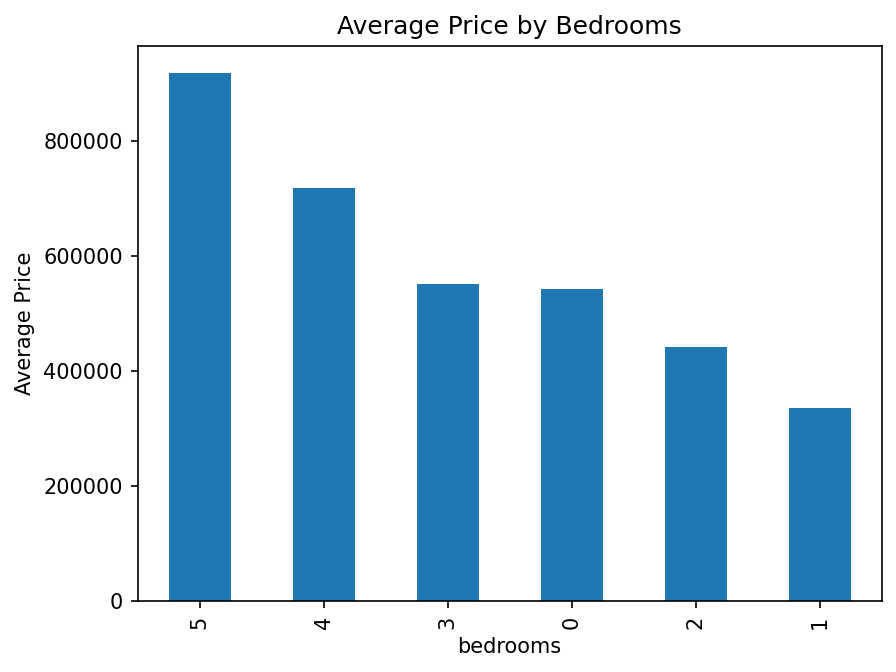
\includegraphics[width=0.45\textwidth]{../imgs/avg_price_by_bedrooms.png}
        \hfill
        
\includegraphics[width=0.45\textwidth]{../imgs/avg_price_by_bedrooms_imputed.png}
    \end{center}



\end{frame}

%------------------------------------------------

\begin{frame}{Distribution of Property Prices}

    %image
    \begin{center}
        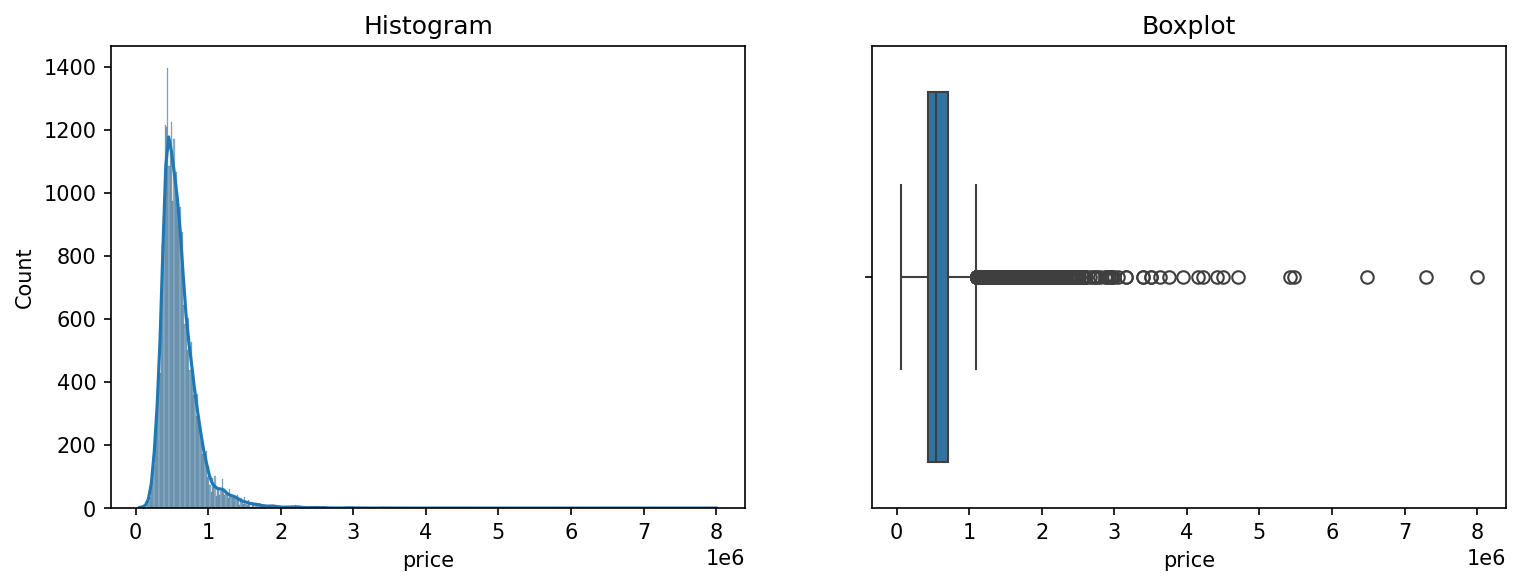
\includegraphics[width=1\textwidth]{../imgs/distribution_price.png}
    \end{center}

    \begin{itemize}

        \item Prices are strongly right-skewed

        \item Presence of very expensive properties

        \item Outliers may affect machine learning models

    \end{itemize}

\end{frame}
%------------------------------------------------

\begin{frame}{Outlier Handling}

    I explored different strategies:

    \begin{itemize}

        \item Keep data unchanged

        \item Remove extreme values using IQR rule:

              \begin{itemize}
                  \item \begin{math}
                            Q1 = 25^{th} \text{ percentile}, Q3 = 75^{th} \text{ percentile}, IQR = Q3 - Q1
                        \end{math}
                  \item Outliers defined as values outside the range: \begin{math}
                            [Q1 - 1.5 \cdot IQR, Q3 + 1.5 \cdot IQR]
                        \end{math}
              \end{itemize}

        \item Apply logarithmic transformation, which is usually effective for right-skewed data

    \end{itemize}

    These approaches were tested during model evaluation. Different models preferred different strategies.

\end{frame}

\begin{frame}{Outlier Handling}{Visual Comparison}
    %two images one above the others, remove vs log_transform, with captions
    \begin{center}
        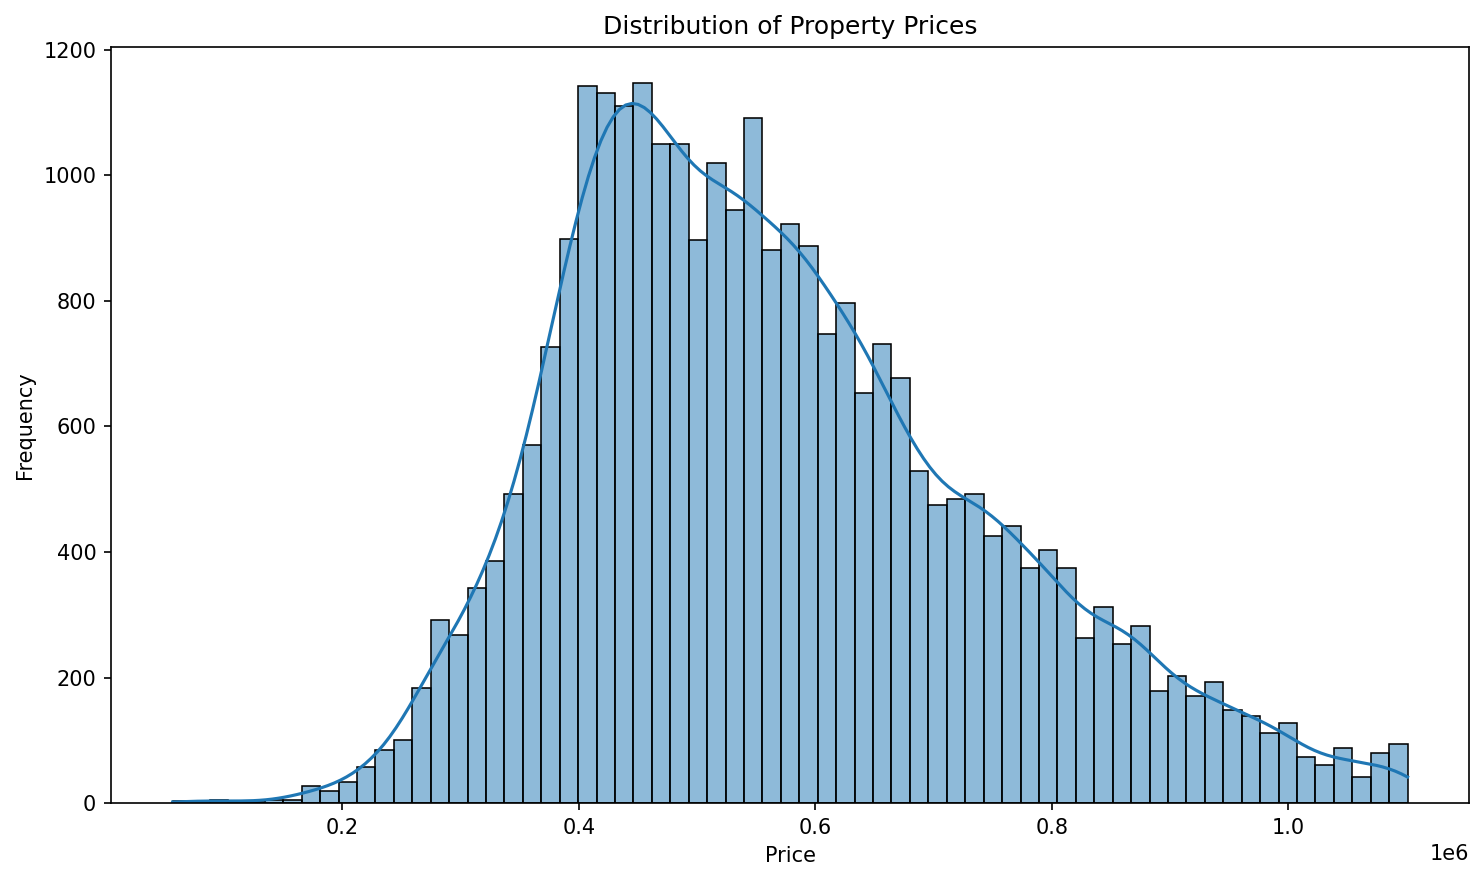
\includegraphics[width=0.49\textwidth]{../imgs/price_distribution_remove.png}
        \vspace{1em}
        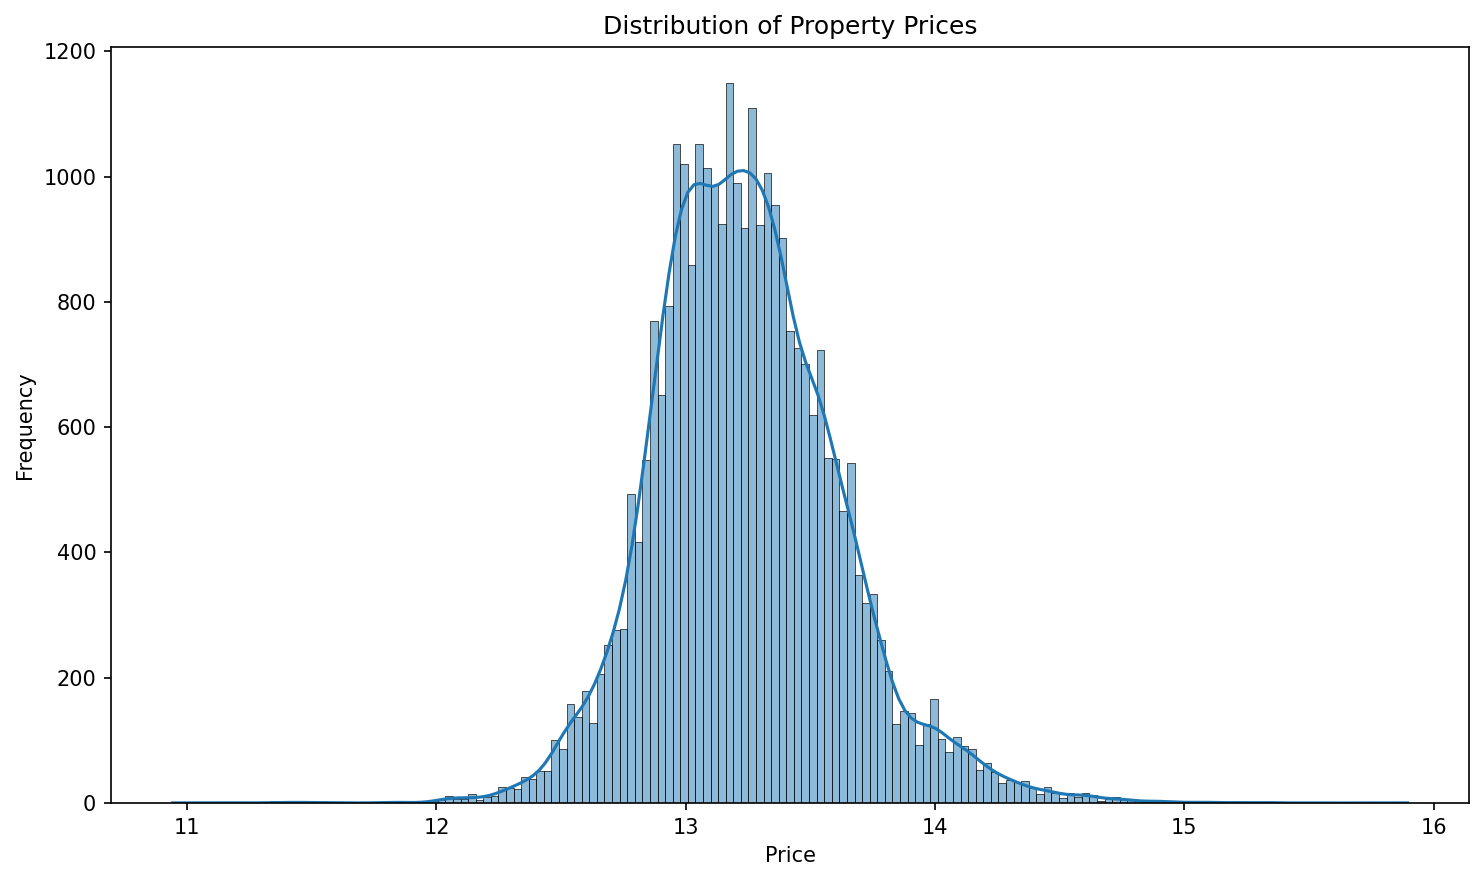
\includegraphics[width=0.49\textwidth]{../imgs/price_distribution_log_transform.png}
    \end{center}
    %CAPTIONS
    \begin{itemize}
        \item Left: Removing outliers using IQR rule
        \item Right: Logarithmic transformation of prices
    \end{itemize}
\end{frame}

%------------------------------------------------
% \begin{frame}{Average Price by Property Type}

%     \begin{itemize}

%         \item Houses tend to be more expensive than units

%         \item Property type is therefore an important explanatory feature

%               \begin{center}
%                   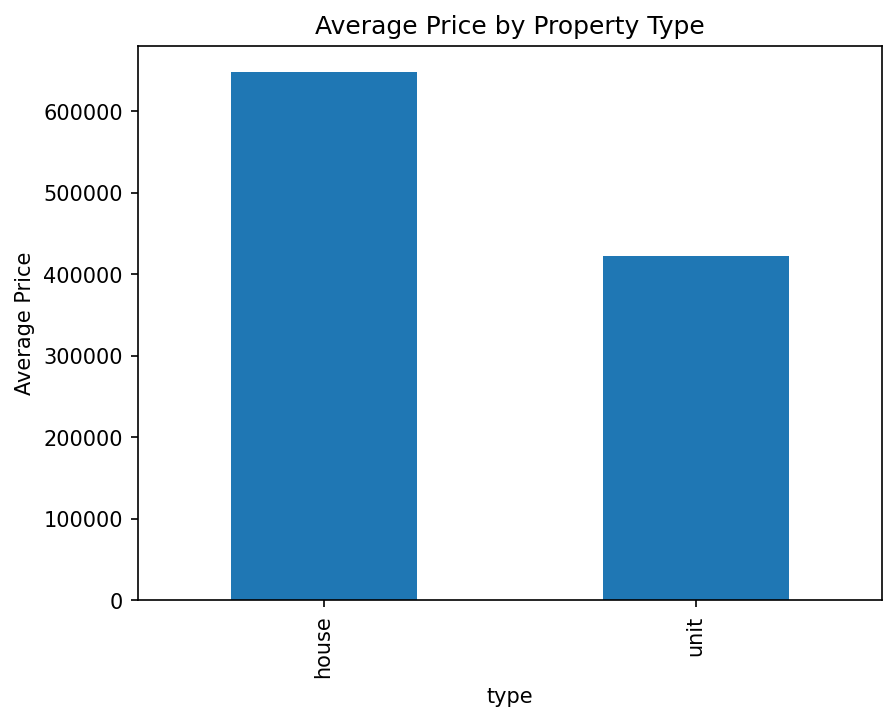
\includegraphics[width=0.6\textwidth]{../imgs/avg_price_by_type.png}
%               \end{center}

%     \end{itemize}

% \end{frame}

%------------------------------------------------
\begin{frame}{From Transactions to Time Series}

    Individual sales were aggregated into monthly statistics:

    \begin{itemize}

        \item median price

        \item number of sales

        \item average bedrooms

        \item house ratio (\begin{math}
                  \text{house ratio} = \frac{\text{number of houses sold}}{\text{total sales}}
              \end{math})

    \end{itemize}

    This creates a \textbf{structured monthly dataset} suitable for forecasting.

\end{frame}

\begin{frame}{Monthly Trends}

    \begin{center}
        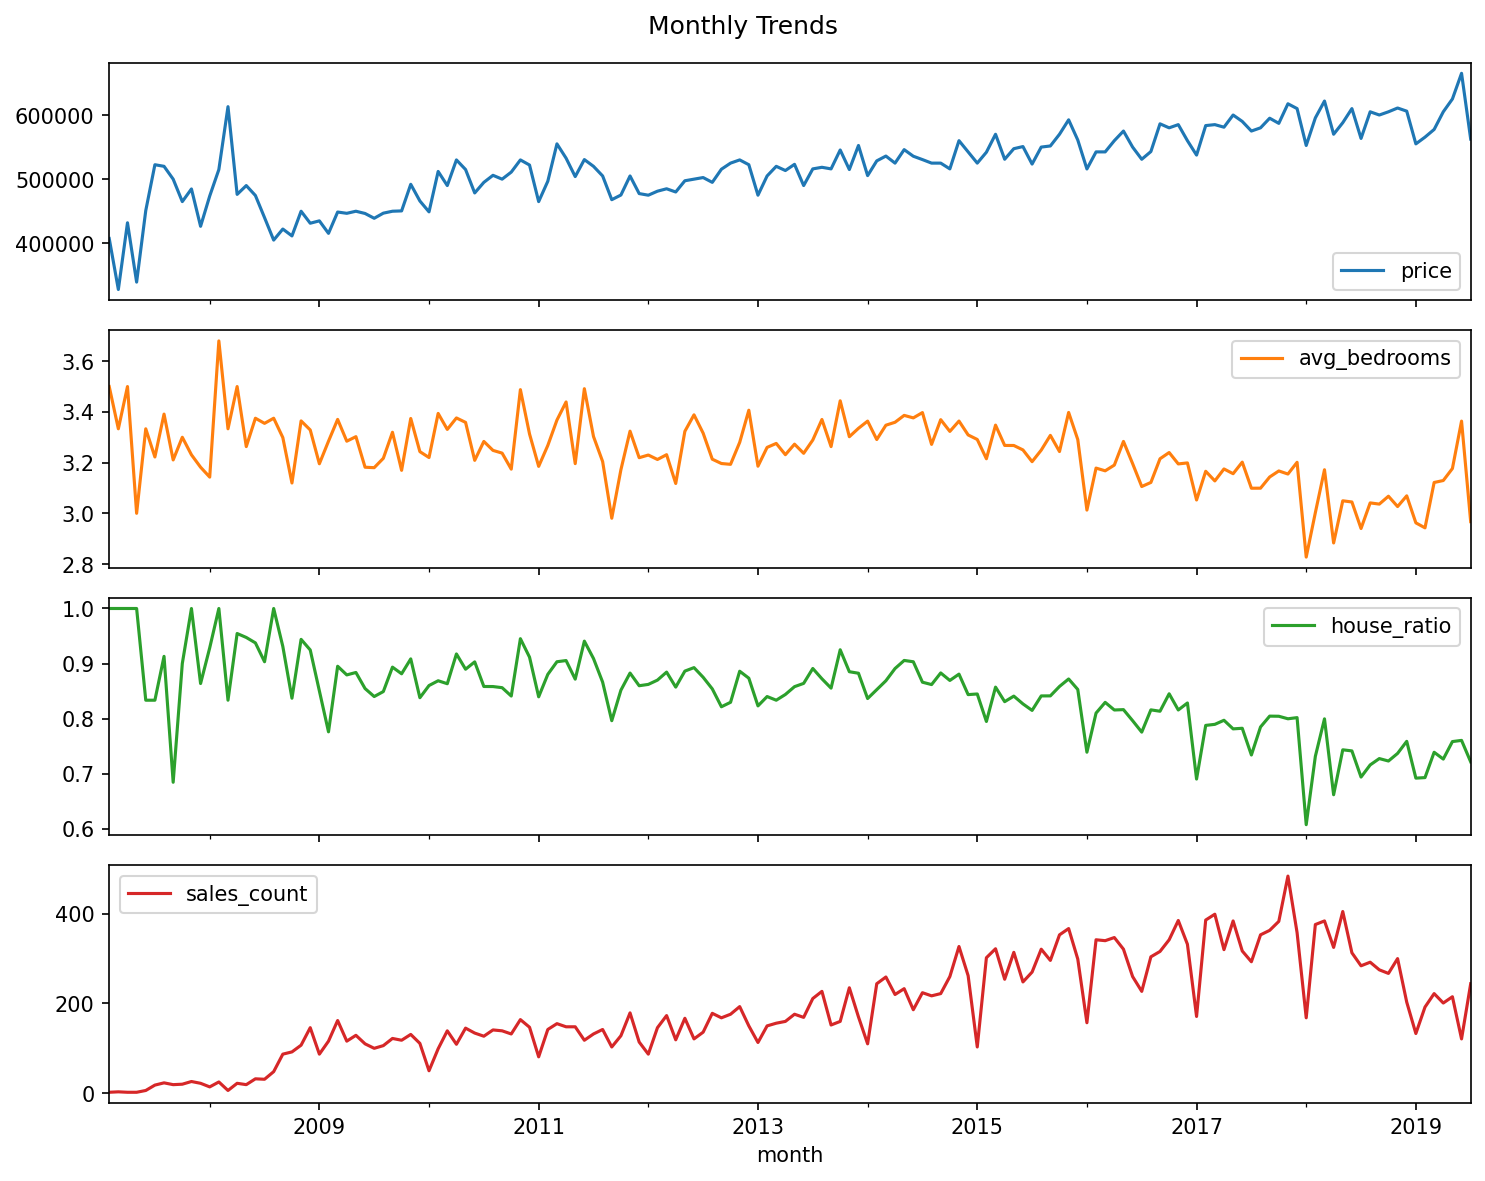
\includegraphics[width=0.75\textwidth]{../imgs/monthly_trends.png}
    \end{center}

\end{frame}

%------------------------------------------------
\begin{frame}{Monthly Price Time Series}

    \begin{center}
        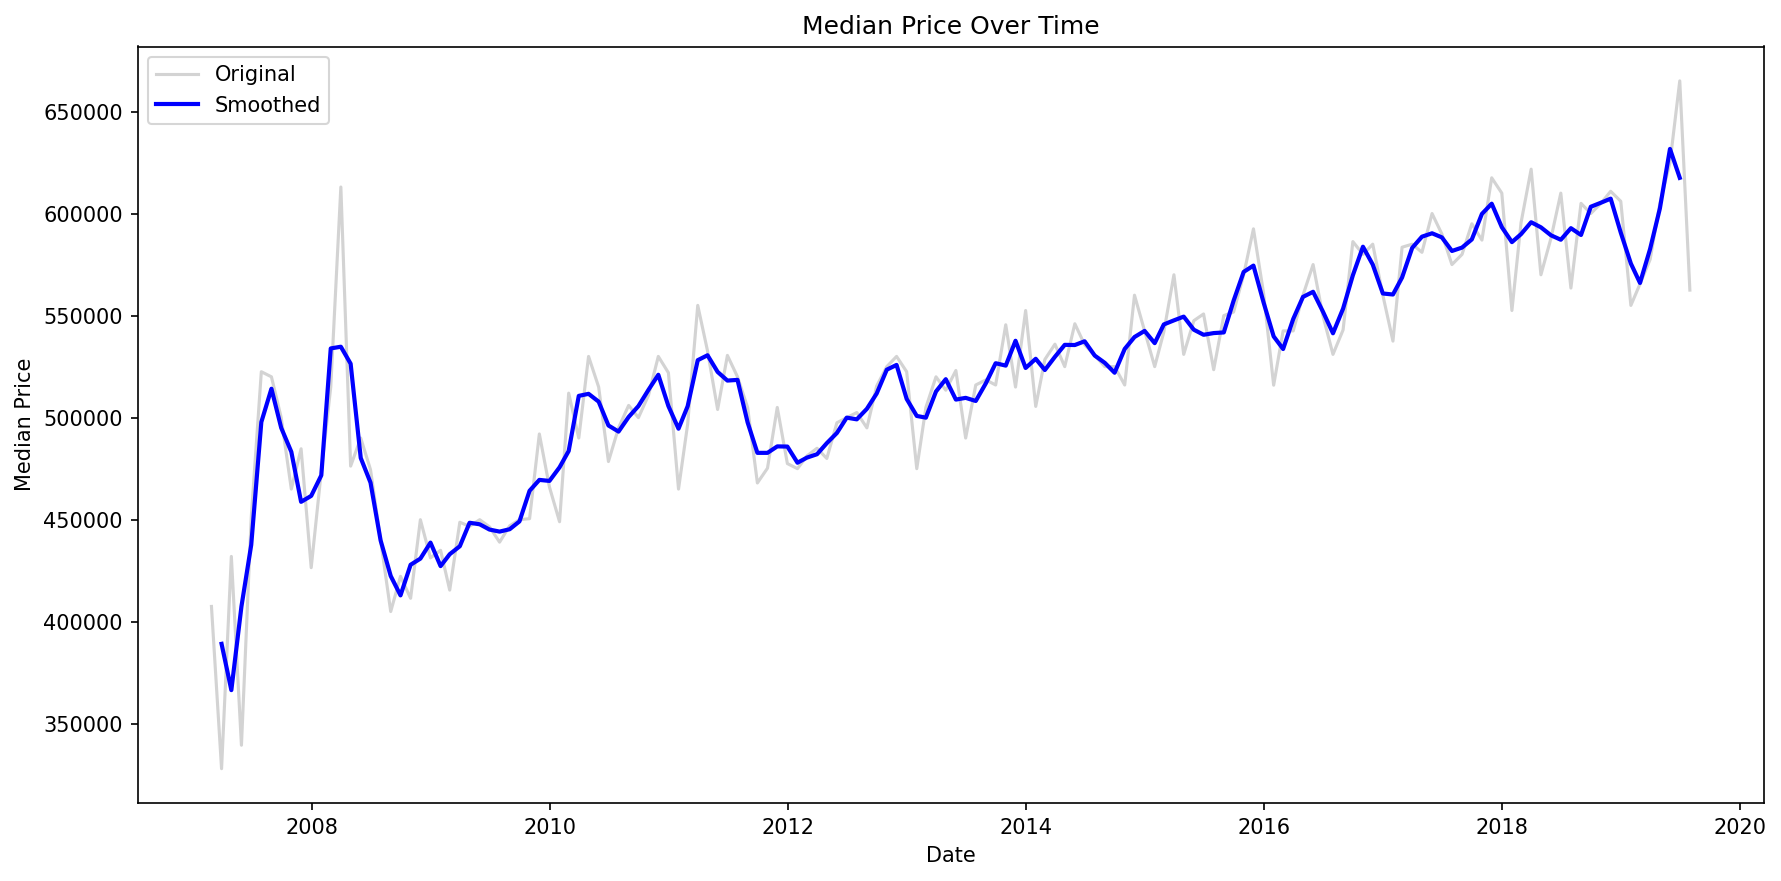
\includegraphics[width=0.9\textwidth]{../imgs/price_trend.png}
    \end{center}

    Observations:

    \begin{itemize}

        \item Clear upward trend in prices over time

        \item Some seasonal fluctuations visible

    \end{itemize}

\end{frame}

%------------------------------------------------
\begin{frame}[fragile]{Seasonal Decomposition}

    \begin{columns}
        \begin{column}{0.35\textwidth}
            \textbf{Additive decomposition:}
            \[
                y_t = T_t + S_t + R_t
            \]
            \begin{itemize}
                \item $T_t$: trend
                \item $S_t$: seasonal
                \item $R_t$: residual
            \end{itemize}
            \vspace{0.5em}
            \begin{lstlisting}[language=Python, basicstyle=\tiny\ttfamily]
from statsmodels.tsa.seasonal \
    import seasonal_decompose

decomp = seasonal_decompose(
    series,
    model='additive',
    period=12
)
            \end{lstlisting}
        \end{column}
        \begin{column}{0.65\textwidth}
            \begin{center}
                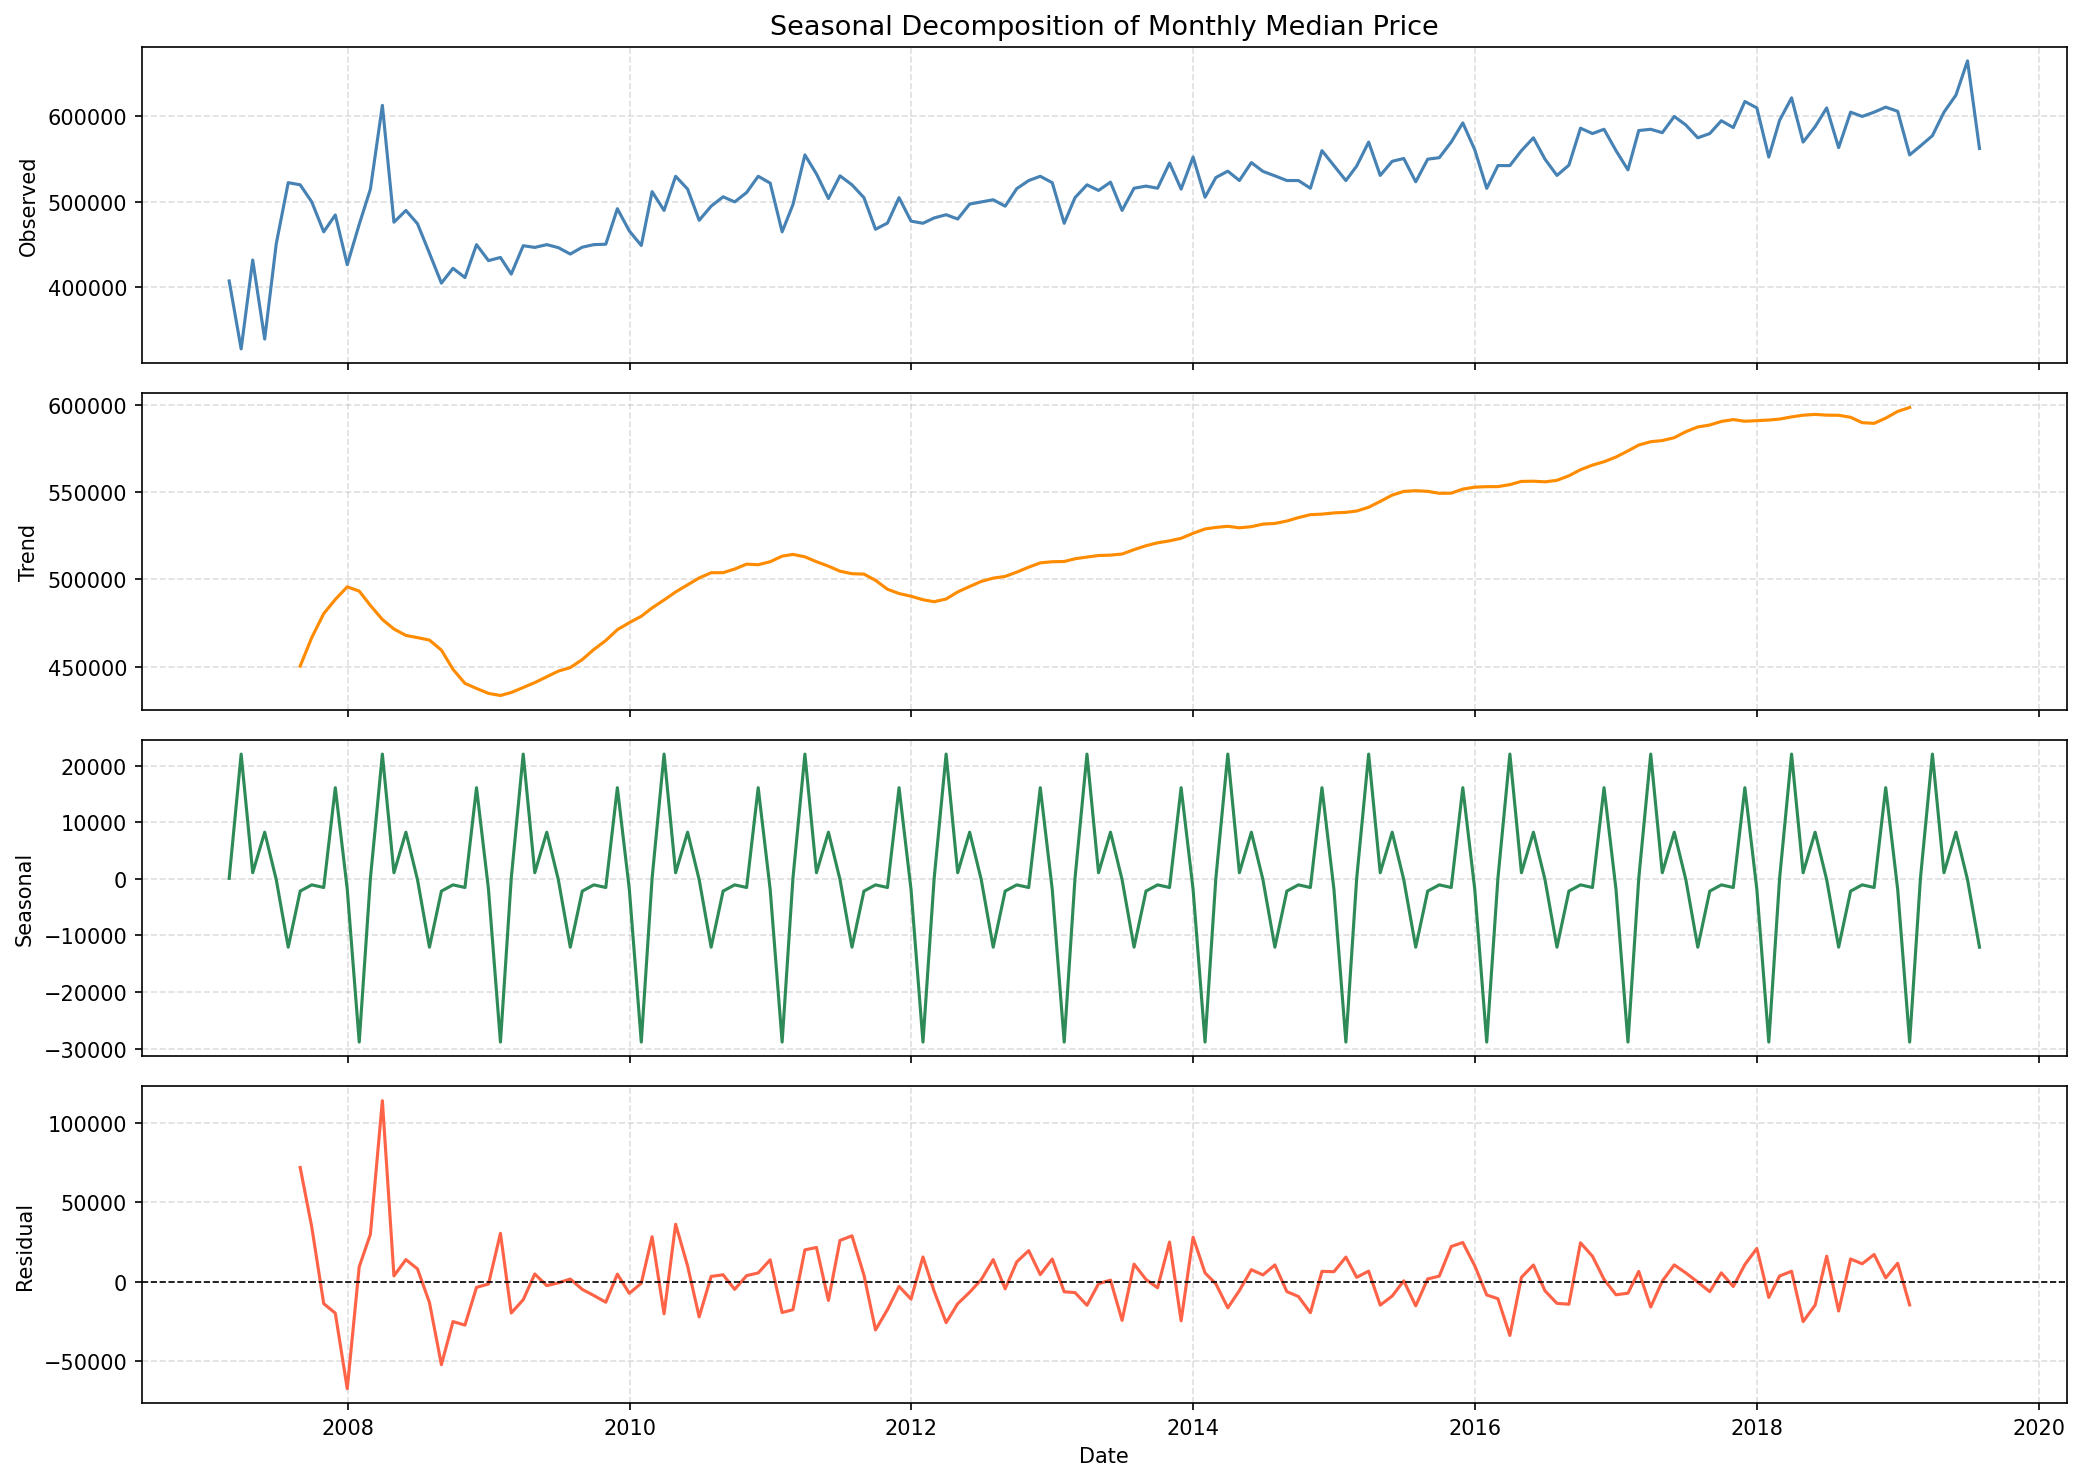
\includegraphics[width=\textwidth]{../imgs/seasonal_decomposition.png}
            \end{center}
        \end{column}
    \end{columns}

\end{frame}

\begin{frame}{Seasonal Decomposition}{Insights}
    \begin{itemize}

        \item Trend component shows long-term price increase

        \item Seasonal component suggests annual cycles

        \item Residual captures irregular fluctuations. These fluctuations may be influenced by external factors not captured in the dataset (e.g., economic conditions, policy changes).
        \item The presence of a strong trend and seasonality indicates that models need to account for these patterns to make accurate forecasts.

    \end{itemize}
\end{frame}

\begin{frame}{Seasonal Decomposition: monthly pattern}

    \begin{center}
        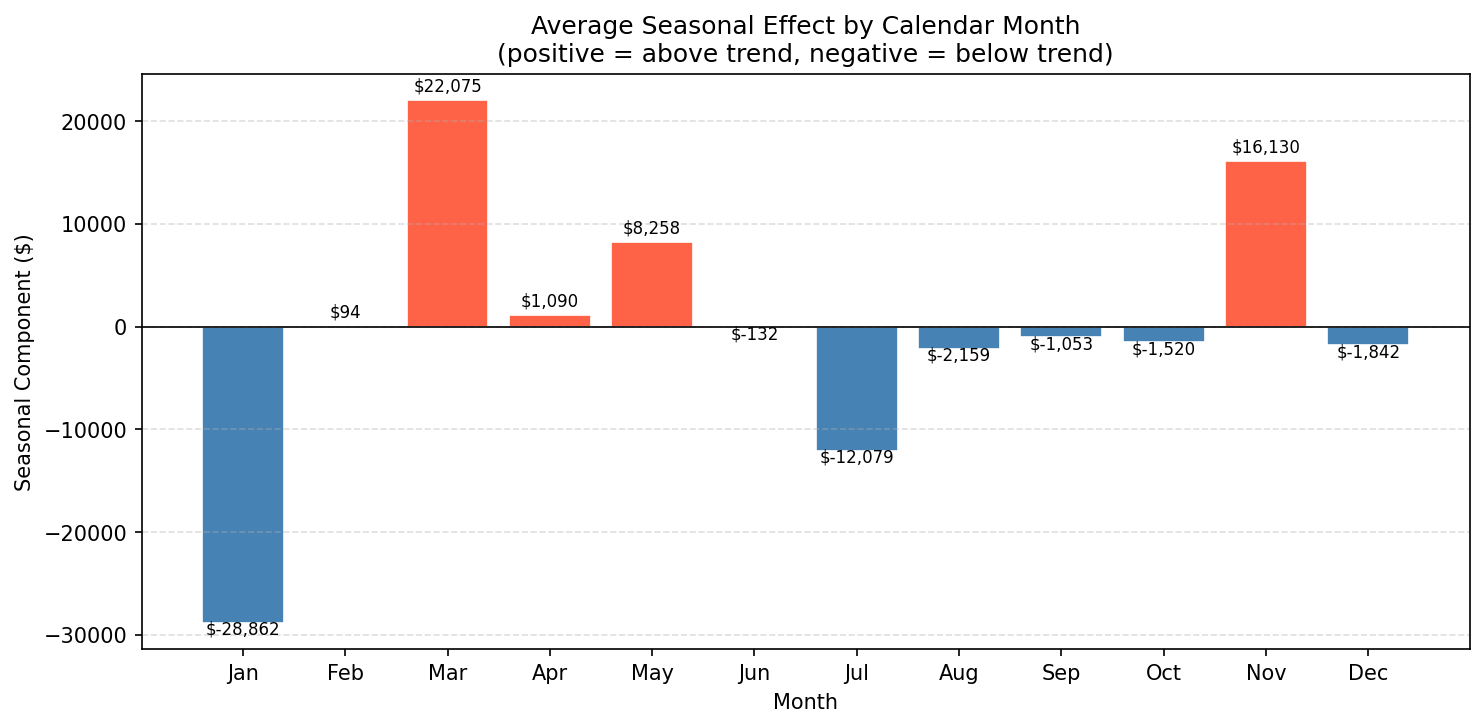
\includegraphics[width=0.75\textwidth]{../imgs/seasonal_pattern_by_month.png}
    \end{center}

    {\small The seasonal component reveals that certain months consistently show higher or lower prices.

    \begin{itemize}

        \item Prices tend to peak in spring and early summer. This makes sense: many buyers prefer to move during warmer months, and families often want to settle before the new school year.

        \item Prices dip in autumn and winter months (except November).

    \end{itemize}}

\end{frame}

%------------------------------------------------
\begin{frame}{Feature Engineering}

    Additional temporal features were introduced:

    \begin{itemize}

        \item Month encoded as cyclical variables (in order for December and January to be close in the feature space, instead of 11 months apart):
              \begin{itemize}
                  \item Sin and Cosine transformations of the month variable.
              \end{itemize}

            \vspace{1em}
              \begin{math}
                  x_{\sin} = \sin\left(2\pi \cdot \frac{x}{\max(x)}\right)
                  \qquad
                  x_{\cos} = \cos\left(2\pi \cdot \frac{x}{\max(x)}\right)
              \end{math}

        %we leave some vertical space
        \vspace{2em}
        \item Scaled year variable representing long-term trend.
    \end{itemize}

    This helps machine learning models capture seasonality.





\end{frame}

\begin{frame}{Cyclical Encoding of Months}
    \begin{center}
        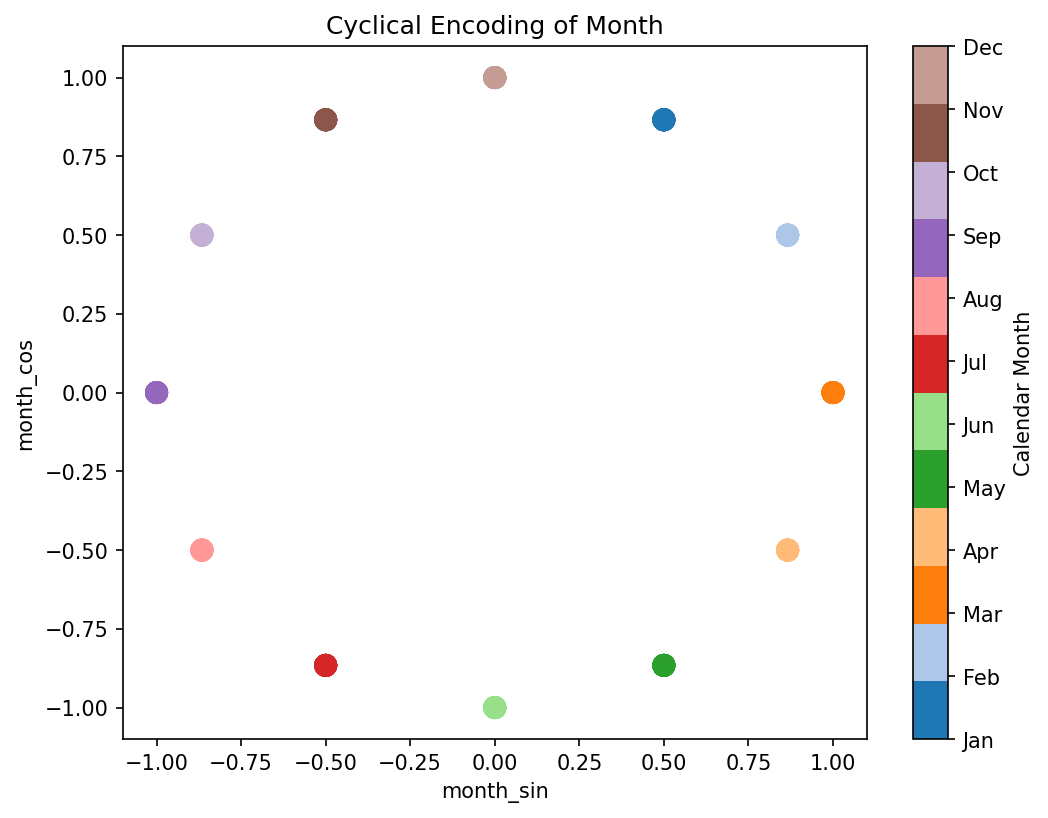
\includegraphics[width=0.75\textwidth]{../imgs/cyclical_encoding_month.png}
    \end{center}
\end{frame}

\begin{frame}{Cyclical Encoding of Months}{Why both sine and cosine?}
    \begin{itemize}
        \item The sine transformation captures the cyclical nature of months, but it is not sufficient to distinguish between all months on its own.

        \item For example, June and December would have the same sine values (because they are symmetric w.r.t equinoxes)

        \item By adding the cosine transformation, we can break this symmetry. Each month will have a unique combination of sine and cosine values, allowing the model to differentiate between all months effectively.
    \end{itemize}

\end{frame}

\begin{frame}
    %big title in the middle
    \begin{center}
        \LARGE{Machine Learning Models}
    \end{center}

\end{frame}

\begin{frame}{Training and Testing Strategy}

    As it is a time series forecasting problem, the data was split
    \textbf{chronologically}, no random shuffling:

    \begin{itemize}
        \item \textbf{Training set:} 2007 -- 2017 \quad (about 70\% of data, although different splits were tested)
        \item \textbf{Testing set:}  2018 -- 2019 \quad (about 30\% of data)
    \end{itemize}

    \medskip

    \textbf{Why chronological split?}
    \begin{itemize}
        \item A chronological split respects the causal order of events:
              the model is only ever trained on information that would
              have been available at prediction time
    \end{itemize}

\end{frame}


\begin{frame}{Model Evaluation}

    Models were evaluated using:

    \begin{itemize}

        \item Root Mean Squared Error (RMSE): we have a direct measure of how close the predictions are to the actual prices, in dollars.

        \item Visual inspection of predicted vs actual price trends

    \end{itemize}

\end{frame}
%------------------------------------------------
\begin{frame}{Random Forest Regressor}

    \begin{itemize}

        \item \textbf{Ensemble of decision trees}, each of which is trained on a random subset of the data and features (this reduces overfitting and improves generalization)
        \item For regression tasks, the final prediction is the average of the predictions from all individual trees. For a single tree, the prediction is made by traversing the tree based on the input features until reaching a leaf node, which contains the predicted value (the average of the target variable for the training samples that fall into that leaf).

        \item Captures non-linear relationships

        \item Represents a good baseline because of its interpretability

    \end{itemize}


\end{frame}

\begin{frame}{Random Forest Regressor: Autocorrelation and Lags}

    \begin{center}
        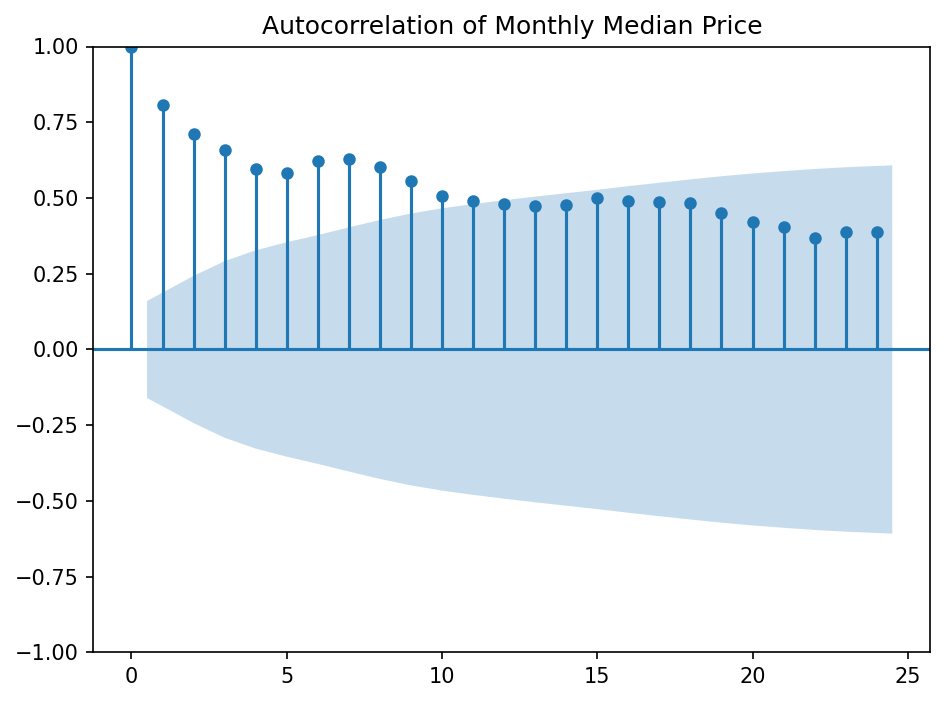
\includegraphics[width=0.65\textwidth]{../imgs/acf.png}
    \end{center}

    The autocorrelation function (ACF) of the monthly price series revealed
    significant correlations up to lag 12.

\end{frame}

\begin{frame}{Recursive Forecasting with Lagged Features}

    To leverage temporal dependencies, lagged price features were created.
    For simplicity, only \textbf{lag 1} and \textbf{lag 12} were used.

    \medskip

    \textbf{Key question:} does using \texttt{price\_lag\_1} at test time
    cause \emph{data leakage} (i.e.\ peeking at future true prices)?

    \medskip

    \textbf{Answer: No}: the model uses \emph{recursive forecasting}:
    each prediction is fed back as input for the next step.
    The true test prices \texttt{y\_test} are \textbf{never accessed}
    inside the forecasting loop.

\end{frame}

\begin{frame}{Recursive Forecasting: Concrete Example}

    \textbf{Setup:} 12 months total, last 3 for testing, feature =
    \texttt{price\_lag\_1}

    \medskip

    \begin{center}
        \begin{tabular}{|c|c|l|}
            \hline
            \textbf{Step}        & \textbf{\texttt{price\_lag\_1} used}            & \textbf{Source}                     \\
            \hline
            Train: Jan $\to$ Sep & true prices                                     & ground truth                        \\
            \hline
            Test Oct             & $p_{\text{Sep}}$ \textnormal{(true)}            & last real training value \checkmark \\
            Test Nov             & $\hat{p}_{\text{Oct}}$ \textnormal{(predicted)} & model's own output \checkmark       \\
            Test Dec             & $\hat{p}_{\text{Nov}}$ \textnormal{(predicted)} & model's own output \checkmark       \\
            \hline
        \end{tabular}
    \end{center}

    \medskip

    The critical line that prevents leakage:
    \begin{center}
        \texttt{history.append(current\_pred)} \quad \emph{(never \texttt{y\_test})}
    \end{center}

    \medskip

    \textbf{Trade-off:} errors \emph{compound} over time: the further
    into the test horizon, the more the model relies on its own
    (potentially noisy) past predictions rather than ground truth.

\end{frame}

%------------------------------------------------


\begin{frame}{Random Forest Results}{All features}

    \begin{center}
        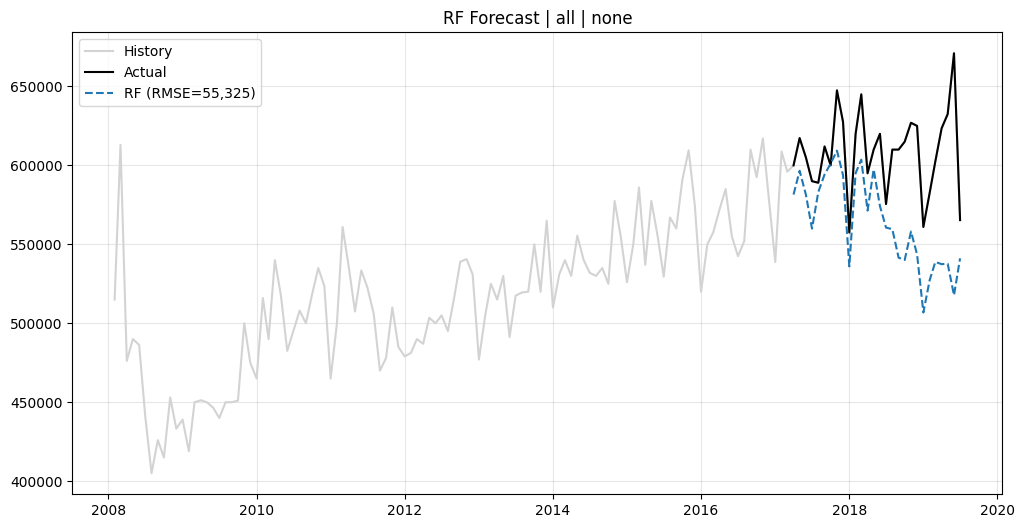
\includegraphics[width=0.70\textwidth]{../imgs/random_forest_all_no_macro.png}
    \end{center}

    Observations:

    \begin{itemize}

        \item Model captures overall trend but underestimates recent price growth: \textbf{why is that?}

    \end{itemize}

\end{frame}

\begin{frame}{Random Forest Results}{Feature importance}

    \begin{center}
        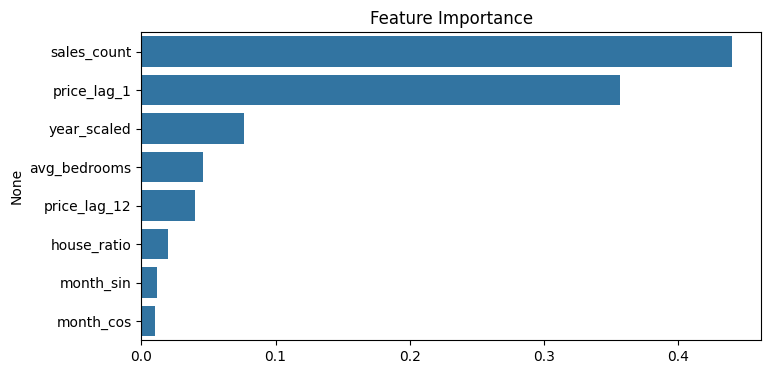
\includegraphics[width=0.95\textwidth]{../imgs/all_features_importance.png}
    \end{center}

    Sales volume and the 1-month lagged price are the most important features.

\end{frame}

\begin{frame}{Random Forest Results}

    \begin{center}
        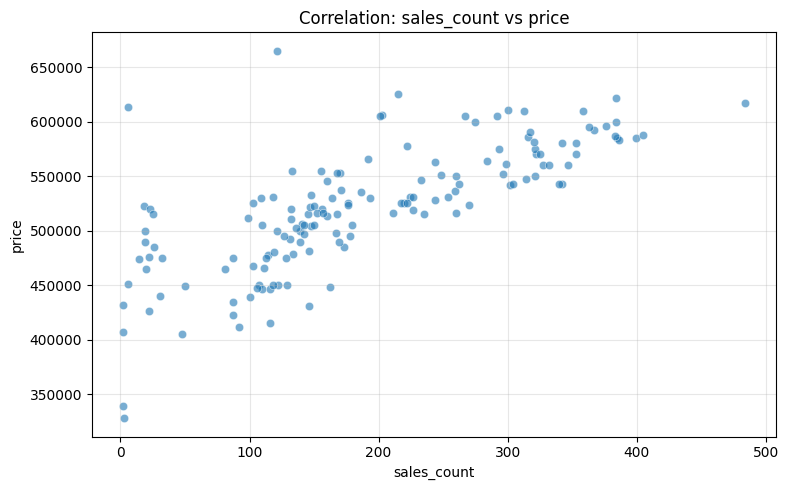
\includegraphics[width=0.65\textwidth]{../imgs/correlation_sales_price.png}
    \end{center}

    \small{There is a strong historical correlation of 0.74. For 85\% of our timeline, sales volume was an excellent proxy for demand, and therefore, price.
        \textbf{Problem}: The model learned a simple rule: lower sales equal a dying market. So, when sales dropped in the final 15\% of our data, the model mathematically assumed prices would follow. They didn't.}

\end{frame}

\begin{frame}{Hypothesis}{More houses than units?}

    \begin{center}
        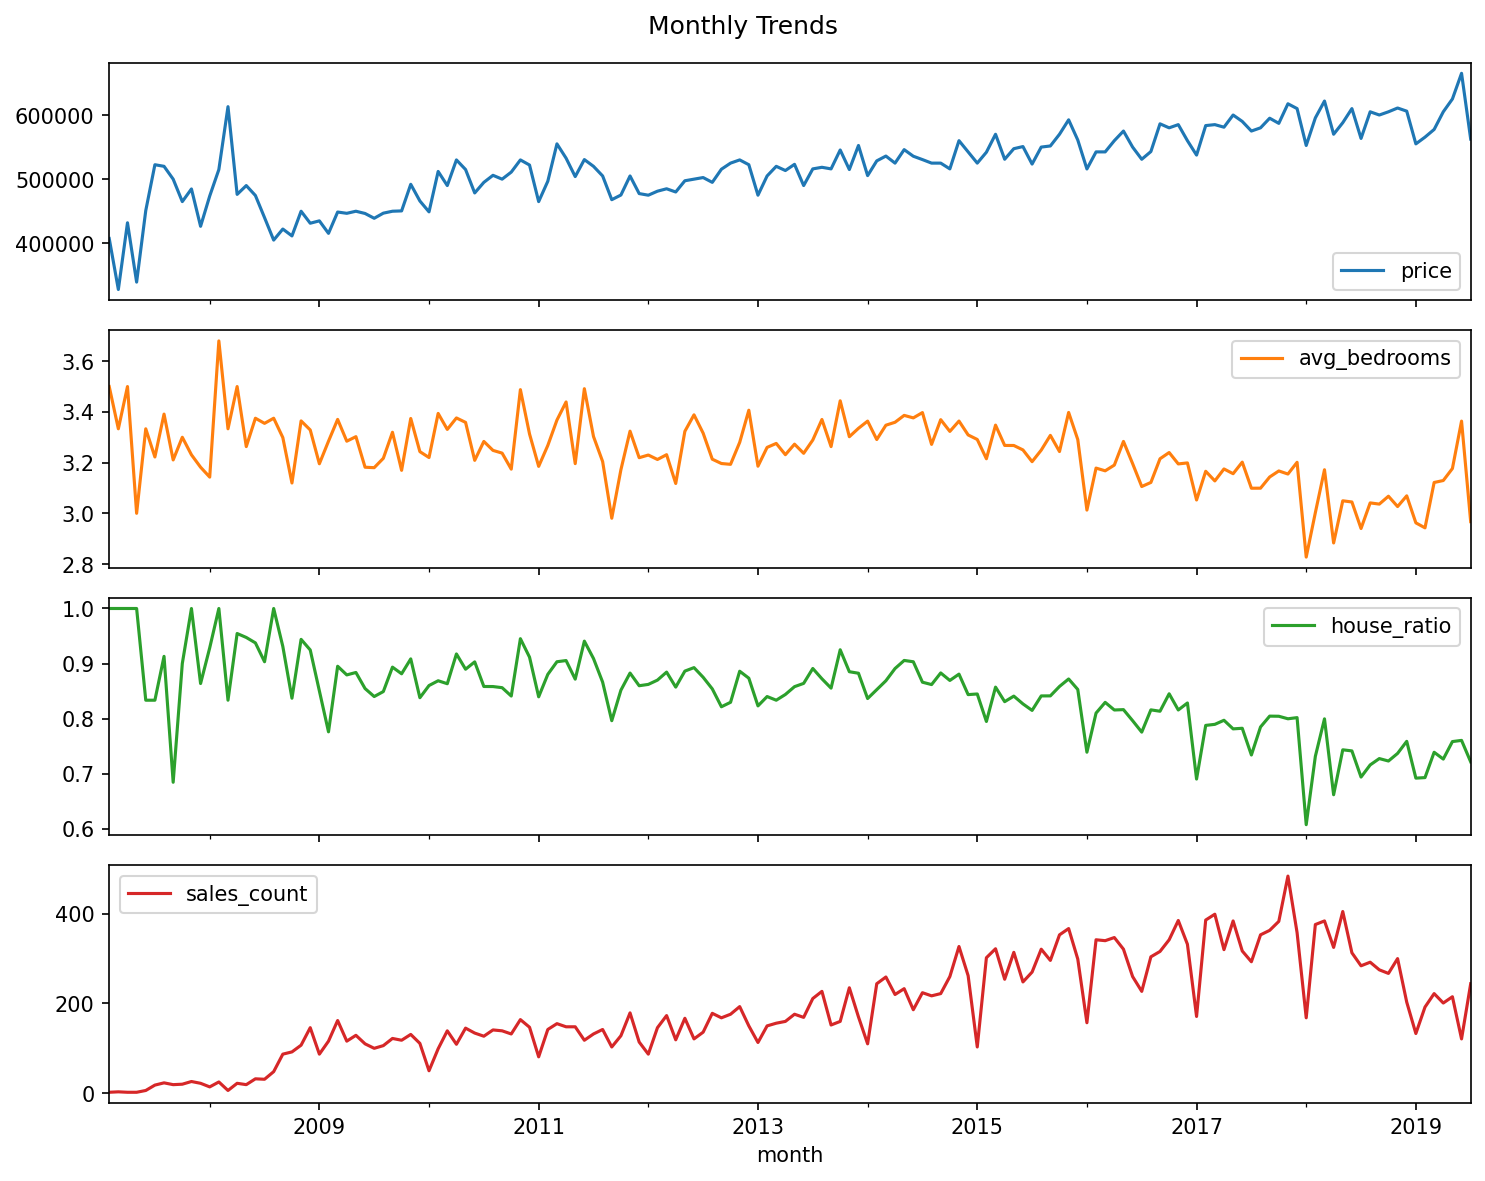
\includegraphics[width=0.60\textwidth]{../imgs/monthly_trends.png}
    \end{center}

    The share of houses (more expensive than units) actually gradually decreased, so this does not explain the price increase.

\end{frame}


\begin{frame}{Hypothesis}{Fewer but more premium-zone houses?}

    \begin{center}
        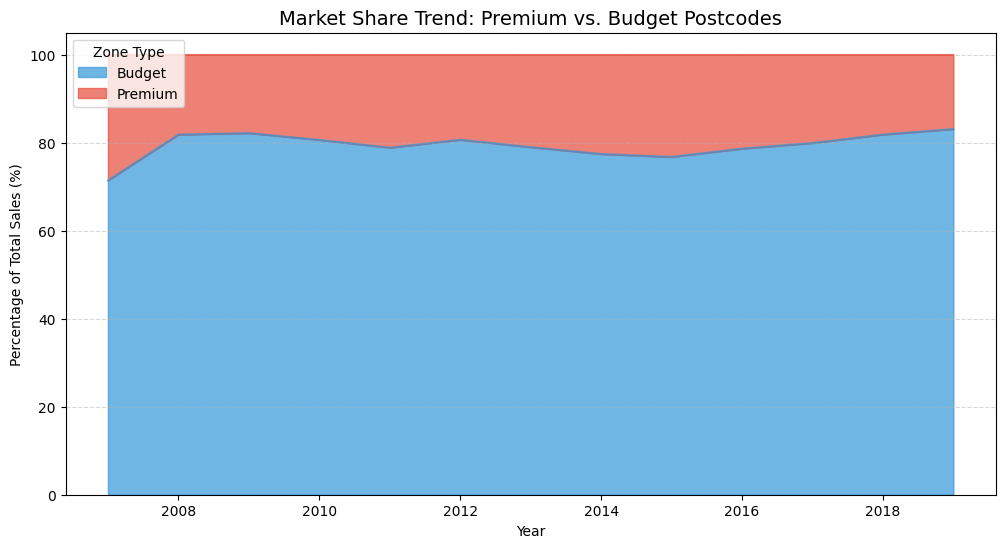
\includegraphics[width=0.75\textwidth]{../imgs/premium_zone.png}
    \end{center}

    The share of sales in top-tier zip codes remained relatively stable. We are not just seeing a luxury market distortion.

\end{frame}

\begin{frame}{Two new features}
    %here we talk about the fact that:
    %  - when mortgage rates go up, sales go down by a lot
    % - when median income goes up, sales go up, and price goes up even faster

    \begin{center}
        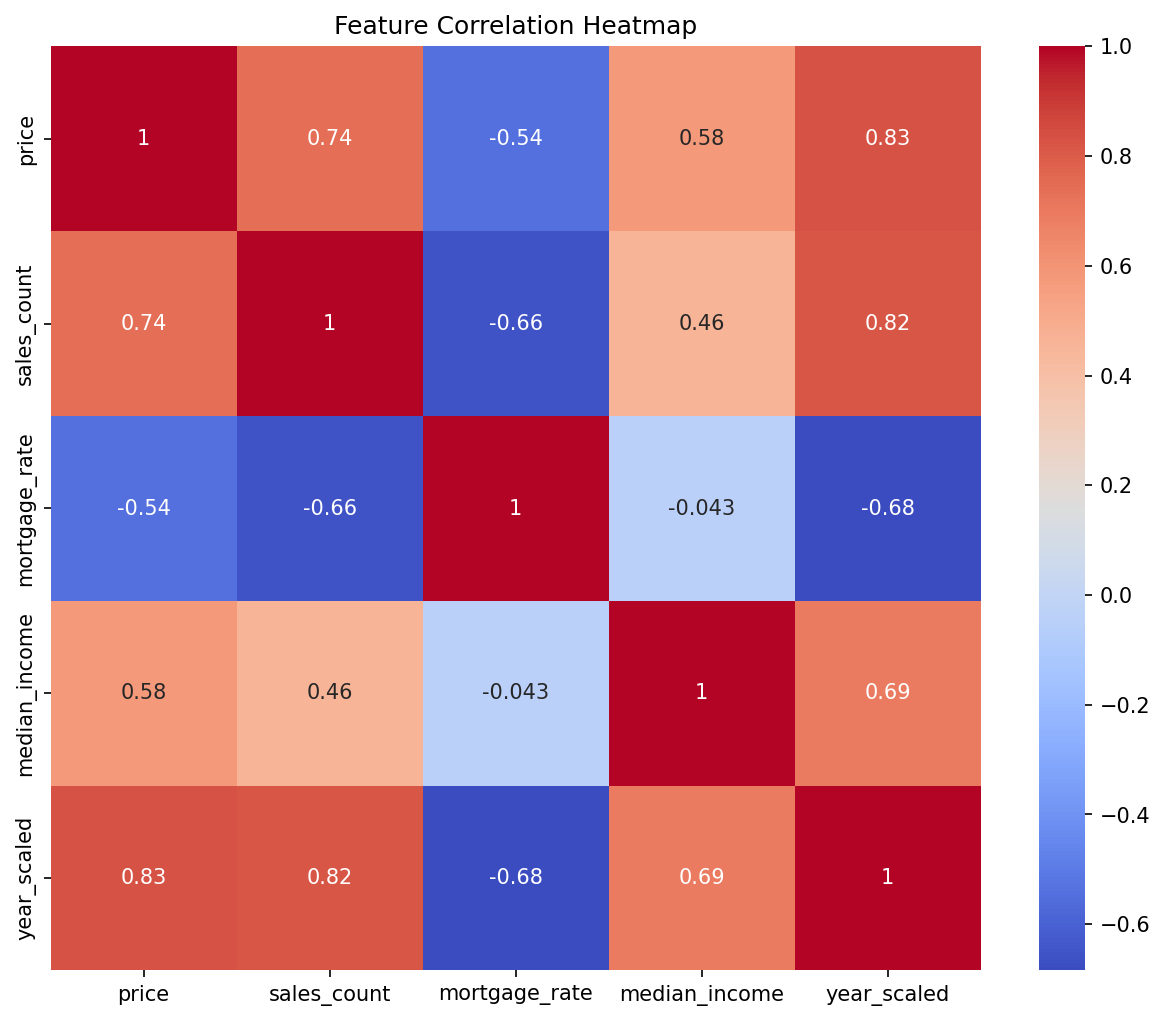
\includegraphics[width=0.65\textwidth]{../imgs/feature_correlation_heatmap_monthly.png}
    \end{center}

\end{frame}



\begin{frame}{Random Forest Results}{We need macroeconomic variables: mortgage rates and family income}

    \begin{center}
        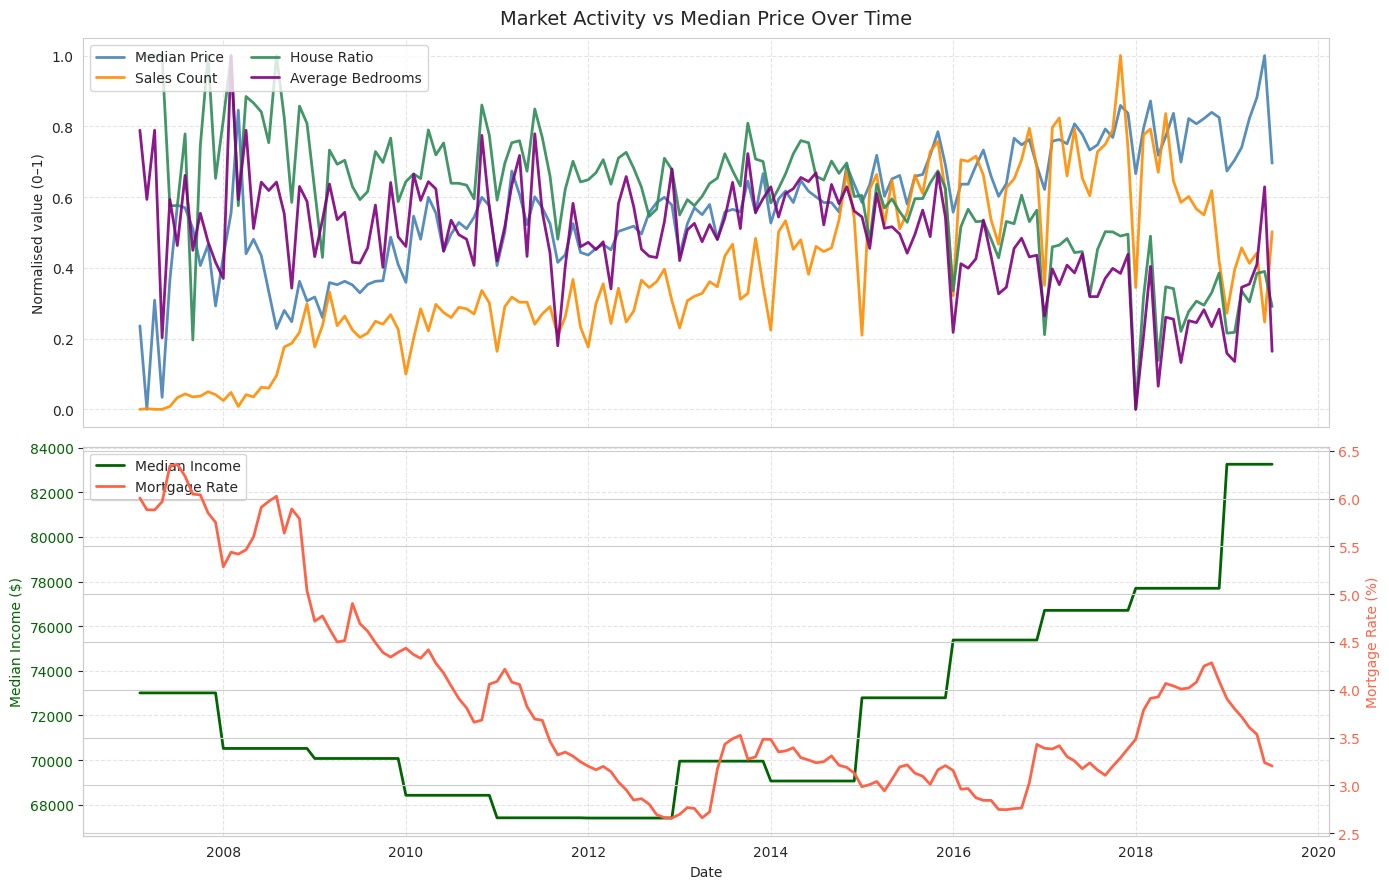
\includegraphics[width=0.9\textwidth]{../imgs/macro_trends_over_time_with_sales.png}
    \end{center}


\end{frame}

\begin{frame}{Macroeconomic Effects}{Interpretation}

    By looking at the trends in later years (where the apparent inconsistency occurs), we can see that:

    \begin{itemize}

        \item Mortgage (negatively correlated with sales and prices) first sharply increased, then decreased. This could have caused a temporary drop in sales, but also a subsequent boost in prices as affordability improved.

        \item Rising family income can also boost prices (demand and supply), even if fewer transactions occur.

        \item These macro factors can explain why prices continued to rise despite declining sales in the later years of our dataset.

    \end{itemize}
\end{frame}

\begin{frame}{Random Forest Results}{With macroeconomic variables and no sales volume}

    \begin{center}
        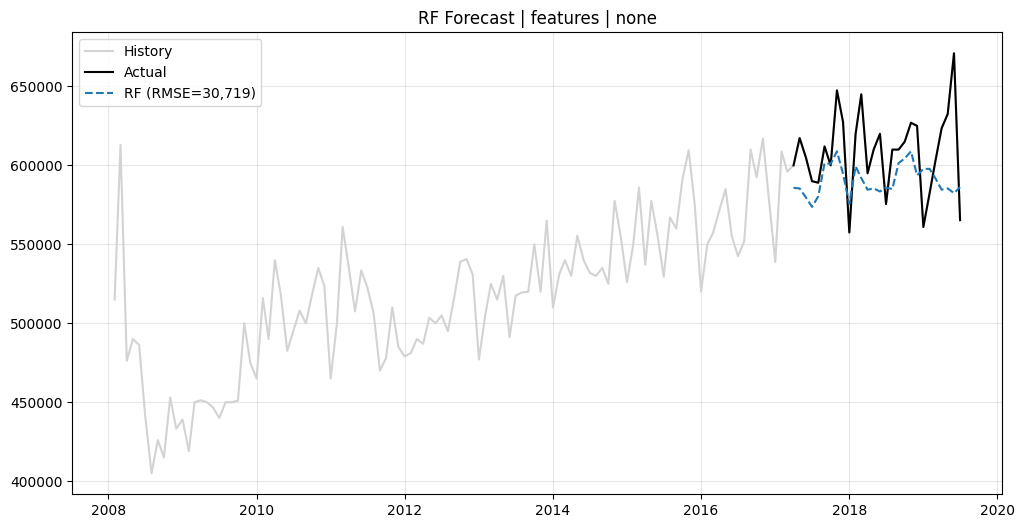
\includegraphics[width=0.75\textwidth]{../imgs/best_features.png}
    \end{center}

    After testing all combinations of features, the best performance was achieved by including macroeconomic variables and excluding sales volume.
    The model now captures the price increase in later years much better.

\end{frame}

\begin{frame}{Random Forest Results}{Feature importance with macro variables}

    \begin{center}
        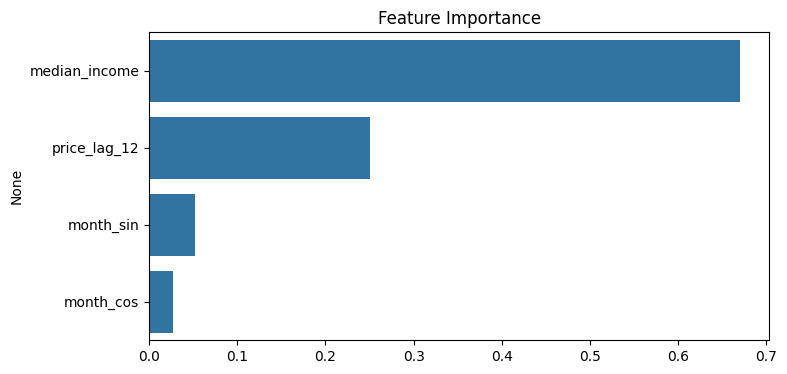
\includegraphics[width=0.95\textwidth]{../imgs/best_features_importance.png}
    \end{center}

    Family income is now among the most important features, while sales volume is no longer used.

\end{frame}

\begin{frame}{A better solution: hybrid model}{Ridge Regression + Random Forest}

    \begin{itemize}
        \item This dataset exhibits a strong \textbf{linear growing trend}, a \textbf{seasonal component}, and a \textbf{residual component} driven by other factors.
    \end{itemize}

    \medskip

    \begin{columns}
        \begin{column}{0.48\textwidth}
            \textbf{Step 1: Ridge Regression}
            \begin{itemize}
                \item Captures the overall long-term trend
            \end{itemize}
        \end{column}
        \begin{column}{0.04\textwidth}
            \centering
            \Large{$+$}
        \end{column}
        \begin{column}{0.48\textwidth}
            \textbf{Step 2: Random Forest}
            \begin{itemize}
                \item Fits the residuals to capture non-linear patterns and seasonality
            \end{itemize}
        \end{column}
    \end{columns}

    \medskip
    \begin{block}{Combined Prediction}
        \[
            \text{Residual} = y - \hat{y}_{\text{Ridge}}
            \qquad \Rightarrow \qquad
            \hat{y} = \hat{y}_{\text{Ridge}} + \hat{y}_{\text{RF}}
        \]
    \end{block}
\end{frame}

\begin{frame}{Hybrid Model Results}

    \begin{center}
        %IMAGE
        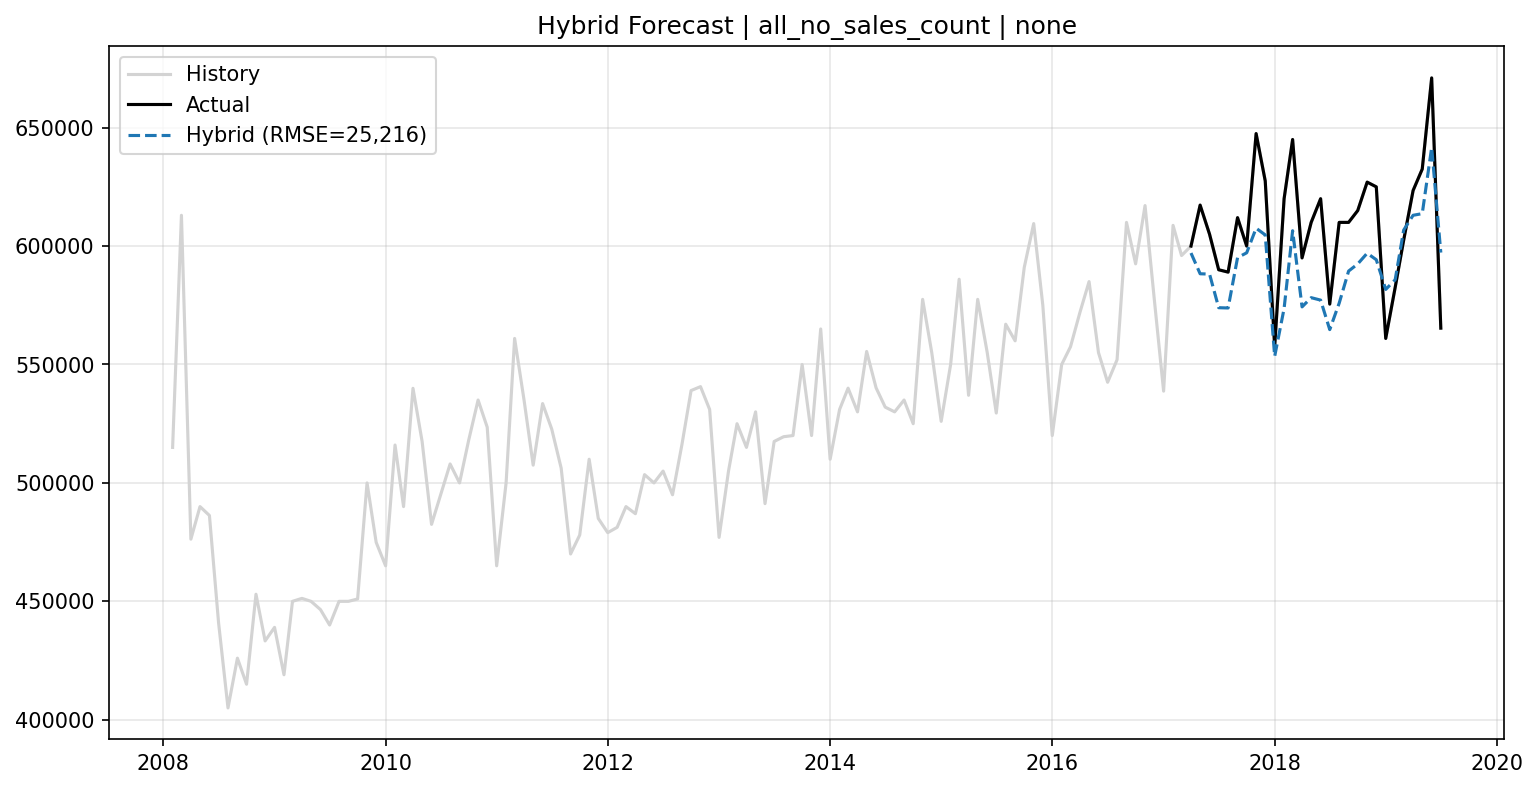
\includegraphics[width=0.75\textwidth]{../imgs/hybrid_forecast_none_all_no_sales_count.png}
    \end{center}

    \begin{itemize}
        \item RMSE is reduced of 17\% compared to the best random forest model, and the price increase in later years is now fully captured.
        \item The 'ups and downs' of the price trend are now much better represented, thanks to the random forest capturing the residuals.
    \end{itemize}

\end{frame}

\begin{frame}{Hybrid Model Results}

    \begin{columns}
        \begin{column}{0.55\textwidth}
            \begin{center}
                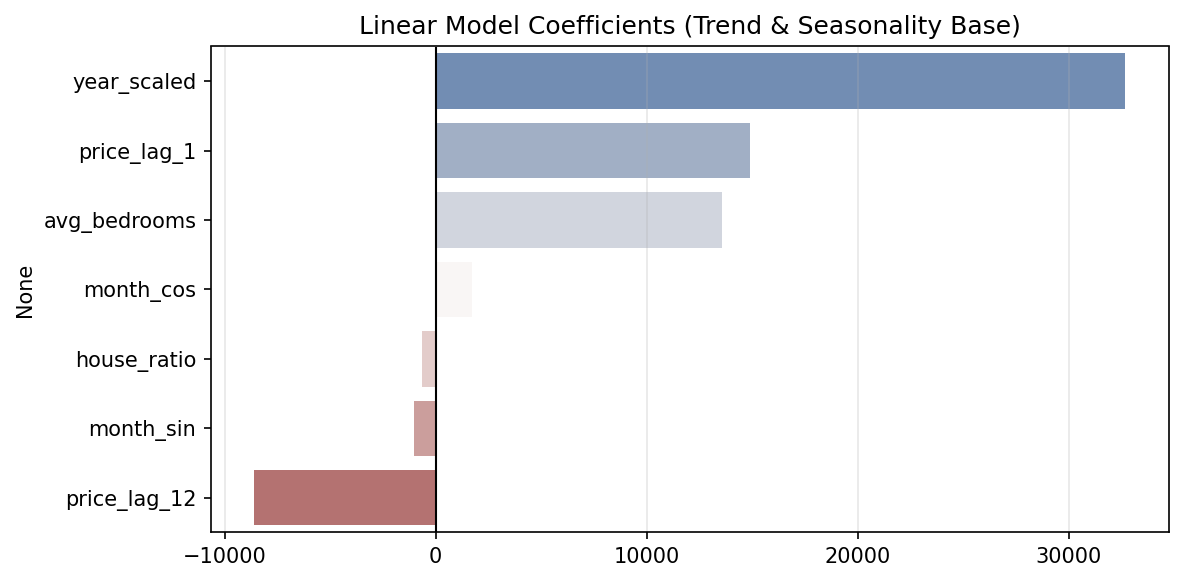
\includegraphics[width=\textwidth]{../imgs/hybrid_linear_coefs_none_all_no_sales_count.png}
            \end{center}
            \begin{center}
                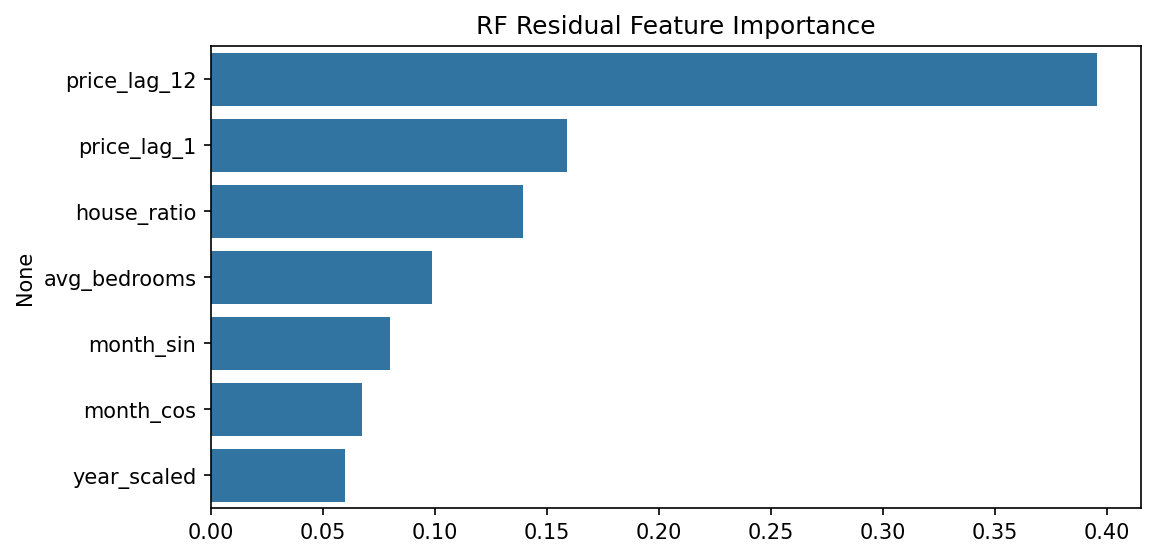
\includegraphics[width=\textwidth]{../imgs/hybrid_importance_none_all_no_sales_count.png}
            \end{center}
        \end{column}
        \begin{column}{0.45\textwidth}
            \small
            \begin{itemize}
                \item \footnotesize{The feature 'year' (as well as the lagged price and the number of bedrooms) is strongly linearly correlated with price, while mortgage rates are negatively correlated. Exactly as expected, and as seen in the correlation matrix.}
                \item  \footnotesize{On the other hand, the house to unit ratio, and the cyclical month features are more important for the random forest, which captures the non-linear and seasonal patterns.}

            \end{itemize}
        \end{column}
    \end{columns}

\end{frame}



%------------------------------------------------
%------------------------------------------------
%------------------------------------------------
%------------------------------------------------
%------------------------------------------------
%------------------------------------------------
%------------------------------------------------
%------------------------------------------------
%------------------------------------------------
%------------------------------------------------

% Slide 1: The Theoretical Appeal of LSTMs
\begin{frame}{Deep Learning Approach: LSTM Networks}
    \begin{block}{Why LSTMs are theoretically a strong solution}
        Long Short-Term Memory (LSTM) networks are designed specifically for sequential data:
    \end{block}

    \begin{itemize}
        \item Through their \textit{Cell State}, they can theoretically maintain a long-term "macro trend" while the \textit{hidden state} captures short-term "ups and downs".
        \item \textbf{The Forget Gate Mechanism:} This allows the network to adaptively decide which historical shocks are noise and which are structural shifts.
        \item \textbf{Non-Linearity:} Unlike traditional models, LSTMs can learn highly complex, non-linear interactions between features like interest rates and price without explicit manual engineering.
    \end{itemize}

\end{frame}

% Slide 2: Empirical Observations & Limitations
\begin{frame}{Empirical Findings: The problem of data scarcity}
    \begin{block}{Observations from implementation}
        While LSTMs are powerful in big data contexts, our specific dataset had important limitations:
    \end{block}

    \begin{itemize}
        \item \textbf{High Variance \& Unreliability:} Due to the small sample size ($\approx$105 months in the training set), the model was extremely sensitive to random weight initialization.
        \item \textbf{Lack of Reproducibility:} Identical training runs yielded significantly different RMSE scores and forecast trajectories.
        \item \textbf{The Smoothing Effect:} The architecture naturally tended to "filter out" the high-frequency fluctuations (wiggles) as noise, resulting in a smoothed average rather than a reactive forecast.
    \end{itemize}

    \begin{alertblock}{Conclusion}
        The model proved too \textbf{stochastic} and \textbf{unstable} for this volume of data.
    \end{alertblock}
\end{frame}

\begin{frame}{LSTM Results: Forecast vs Actual}

    \begin{center}
        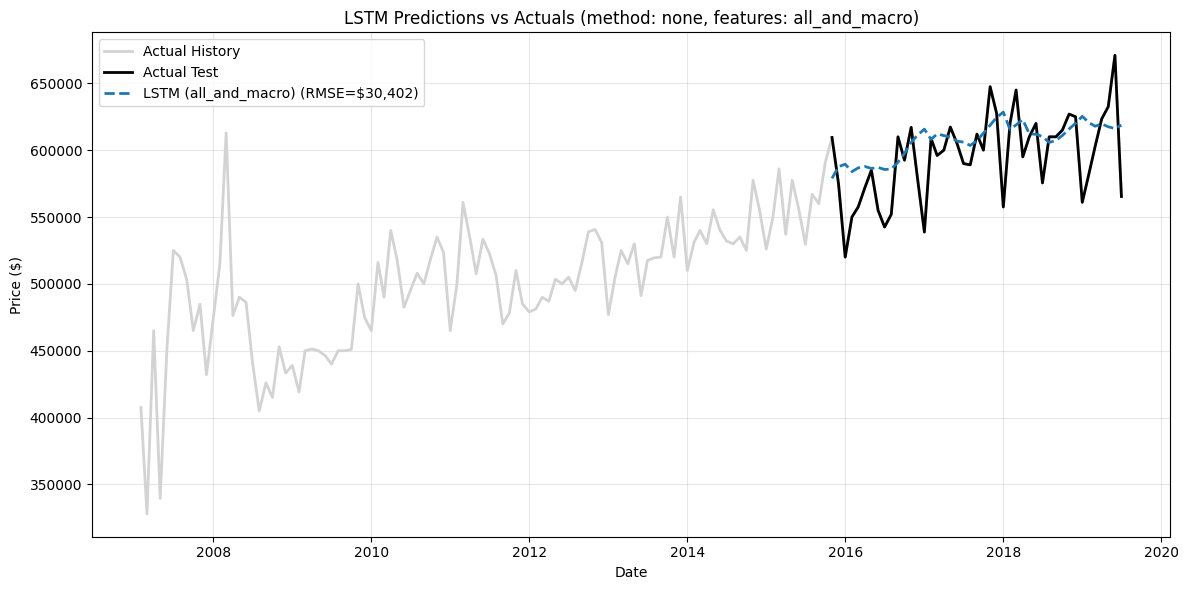
\includegraphics[width=0.9\textwidth]{../imgs/lstm_output.png}
    \end{center}

\end{frame}

\begin{frame}{LSTM Results: SHAP Feature Importance}

    \begin{center}
        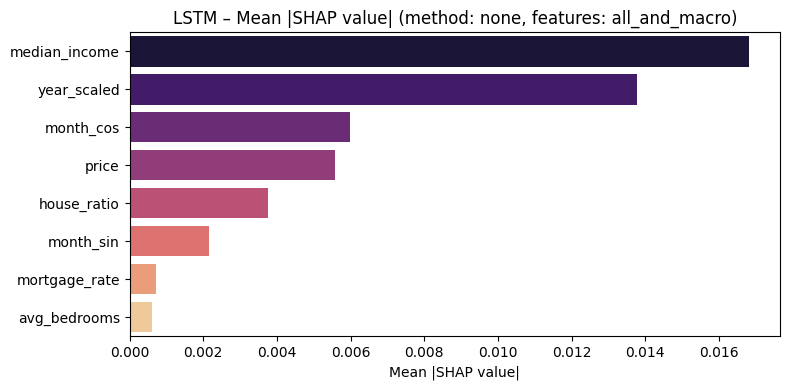
\includegraphics[width=0.9\textwidth]{../imgs/lstm_shap.png}
    \end{center}

\end{frame}

%------------------------------------------------
%------------------------------------------------
%------------------------------------------------
%------------------------------------------------
%------------------------------------------------
%------------------------------------------------
%------------------------------------------------
%------------------------------------------------
%------------------------------------------------
%------------------------------------------------

%------------------------------------------------
\begin{frame}{What is SARIMAX?}

    SARIMAX = \textbf{Seasonal AutoRegressive Integrated Moving Average} with \textbf{eXogenous variables}.

    \begin{itemize}
        \item Time series forecasting statistical model (can be used with limited data, it is not a data-hungry deep learning model)
        \item Combines regression and autoregressive dynamics
        \item Captures:
              \begin{itemize}
                  \item temporal dependence
                  \item seasonality
                  \item external predictors
              \end{itemize}
    \end{itemize}

    Model structure:

    \[
        y_t = AR + MA + Seasonal + Exogenous + \epsilon
    \]

\end{frame}

\begin{frame}{Handling Non-Stationary Data}

    Time series often contain trends:

    \begin{itemize}
        \item Housing prices increase over time
        \item Data is therefore non-stationary
    \end{itemize}

    SARIMAX solves this using \textbf{differencing}:

    \[
        y'_t = y_t - y_{t-1}
    \]

    This removes the trend and makes the series stationary.

    The model then learns patterns in the stationary series.
    Then, predictions are transformed back to the original scale by reversing the differencing:
    \[
        \hat{y}_t = \hat{y}'_t + y_{t-1}
    \]

\end{frame}



\begin{frame}{Model Structure}

    Selected model:

    \[
        \text{SARIMAX}
        \!\underbrace{(
        \underbrace{2}_{\text{AR}},\,
        \underbrace{1}_{\text{I}},\,
        \underbrace{0}_{\text{MA}}
        )}_{\text{non-seasonal}}
        \times
        \underbrace{(
        \underbrace{1}_{\text{SAR}},\,
        \underbrace{0}_{\text{SI}},\,
        \underbrace{1}_{\text{SMA}}
        )_{\underbrace{12}_{\text{period}}}}_{\text{seasonal}}
    \] Meaning:

    \begin{itemize}
        \item AR(2): uses two previous observations (lags 1 and 2)
        \item I(1): first difference applied to achieve stationarity
        \item MA(0): no moving average component (past errors not used)
        \item Seasonal AR(1): yearly dependence
        \item Seasonal differencing not needed (seasonality is stable)
        \item Seasonal MA(1): seasonal error correction
        \item Period = 12 months
    \end{itemize}

\end{frame}

\begin{frame}{How does SARIMAX fit the data?}

    \begin{itemize}
        \item The model identifies the best combination of AR, I, MA, and seasonal parameters by minimizing the AIC (Akaike Information Criterion).
              \begin{itemize}
                  \item AIC balances model fit and complexity, penalizing overfitting.
              \end{itemize}
        \item It captures both short-term dependencies (AR and MA) and long-term seasonal patterns (seasonal AR and MA).
        \item Exogenous variables can be included to account for external factors influencing prices. In our case, we included the features of the dataset.
    \end{itemize}

\end{frame}

\begin{frame}{SARIMAX Results: Forecast vs Actual}

    \begin{center}
        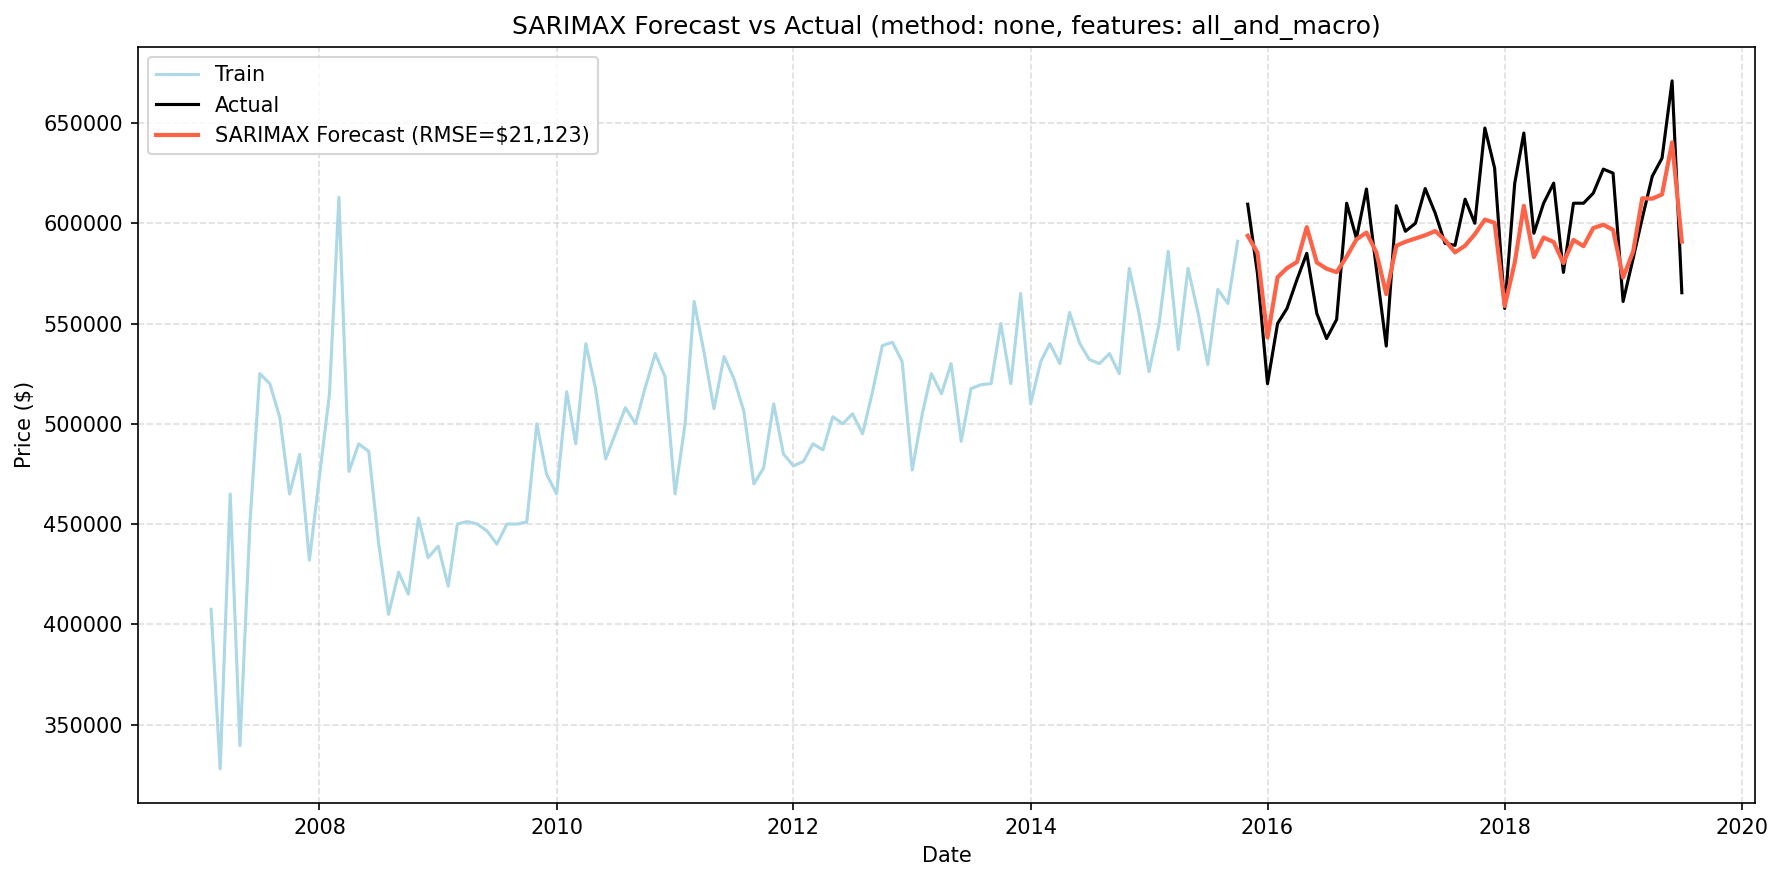
\includegraphics[width=0.9\textwidth]{../imgs/sarimax_forecast_none_all_and_macro.png}
    \end{center}

    MAPE (Mean Absolute Percentage Error) is 3.06\%, which is a very good result.

\end{frame}

% \begin{frame}{SARIMAX Results: Coefficients}

%     \begin{center}
%         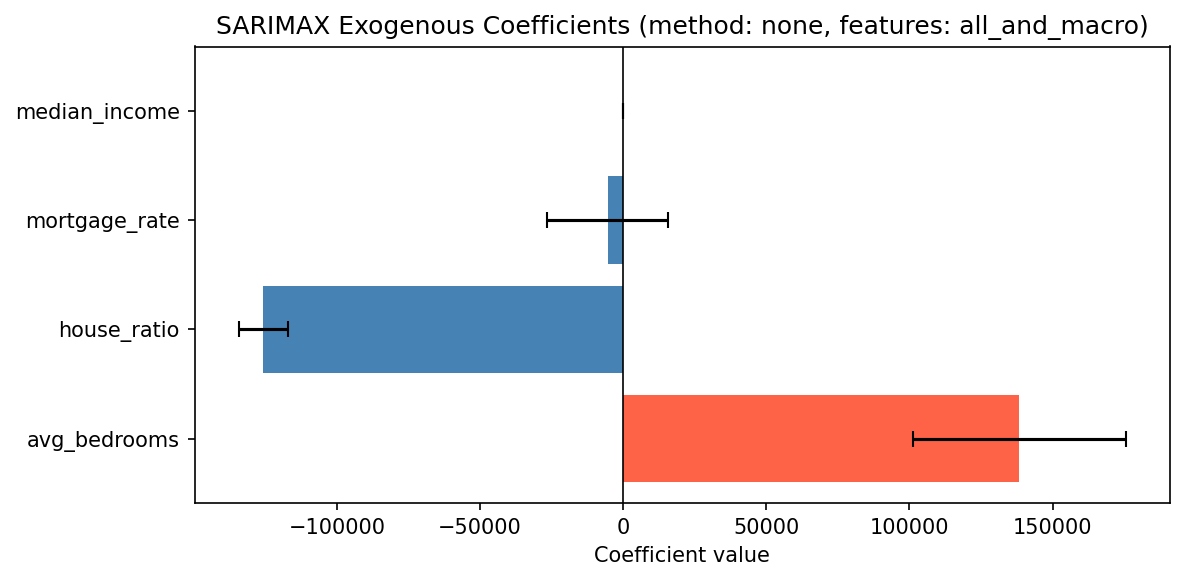
\includegraphics[width=0.9\textwidth]{../imgs/sarimax_coefficients_none_all_and_macro.png}
%     \end{center}

% \end{frame}

%------------------------------------------------

%------------------------------------------------
\begin{frame}{Conclusion}

    \begin{itemize}

        \item Machine learning models can effectively forecast housing prices

        \item Understanding model errors can reveal deeper insights

        \item Integrating macroeconomic indicators significantly improves interpretation

    \end{itemize}

    Future work:

    \begin{itemize}

        \item incorporate additional economic indicators

        \item explore spatial models

        \item test alternative deep learning architectures

    \end{itemize}

\end{frame}

%------------------------------------------------
\begin{frame}{References}

    \begin{itemize}

        \item Kaggle Housing Sales Dataset

        \item Housing Market Forecasting Literature

        \item Time Series Forecasting with Decomposition

    \end{itemize}

\end{frame}

%------------------------------------------------
\end{document}
